\chapter{函数的极限和连续函数的性质}

\section{函数的极限}
\subsection{函数极限的概念}

在第四册下,我们研究了数列的极限,数列是一种特殊的函数,这里的自变数$n$取自然数列$1, 2, 3,\ldots,n,\ldots$的值,现在我们来研究更一般的情形,即函数$f(x)$随$x$连续变化而变化的情形,下面转到一般函数的极限.

\begin{blk}{定义1}
    如果$x$通过任何一个无限增大的数列$\{x_n\}$, 对应的函数值数列
$f (x_1 ) ,f (x_2) , \ldots,f (x_n ) ,\ldots$
都以定数$\ell$为它的极限,就说函数$f(x)$, 当$x\to +\infty$时,以$\ell$为极限,记作
\begin{equation}
    \lim_{x\to+\infty}f(x)=\ell\qquad \text{或}\qquad f(x)\to \ell\quad (x\to +\infty)
\end{equation}
\end{blk}
 
从几何上看,极限式(1.1)表示随着$x$无限增大,曲线$y=f(x)$以直线$\ell$为渐近线(图1.1).
\begin{figure}[htp]
    \centering
\begin{tikzpicture}[>=latex]
\draw[->](-3,0)--(5,0)node[right]{$x$};  
\draw[->](0,-1)--(0,3)node[right]{$y$};    
\draw[thick](-3,1)--(5,1)node[right]{$y=\ell$};
\draw[very thick, rounded corners=10pt](-3,.1) --(-1.5,.3) --(-.5,.8) --(1,1.5) --(2.5,.7) -- (3,1.2)--(3.5,.8) --(4.5,1.05);
\node at (0,0)[below right]{$O$};

\end{tikzpicture}
    \caption{}
\end{figure}

类似地,可以定义函数极限$\Lim_{x\to -\infty} f(x)=\ell$, 这时,变量
$x$通过代数值无限地变小,而绝对值无限地增大的任何一个数列$\{x_n\}$.

如果函数$f(x)$当$x\to+\infty$和$x\to-\infty$时,都以定值为极限,就说$f(x)$当$x\to \infty$时,以定值$\ell$为极限,记作$\Lim_{x\to\infty}f(x)=\ell$, 或者$f(x)\to \ell\; (x\to\infty)$.

\begin{example}
    证明$\Lim_{x\to\infty}\frac{1}{x}=0$
\end{example}

\begin{proof}
任何数列$\{x_n\}$的值$x_1,x_2,\ldots,x_n,\ldots$趋向于$+\infty$或$-\infty$时,对应的函数数列
\[\frac{1}{x_1},\frac{1}{x_2},\ldots, \frac{1}{x_n},\ldots\]
的绝对值$\left|\frac{1}{x_n}\right|$便趋向于零,即
    \[\lim_{n\to\infty}\left|\frac{1}{x_n}\right|=0\]
    从而$\Lim_{x\to\infty}\frac{1}{x}=0$
\end{proof}

\begin{example}
证明函数$\sin x$, 当$x\to\infty$时,没有极限.
\end{example}

\begin{proof}
令自变量$x$取数列$x_n=-\frac{\pi}{2}+2n\pi\quad (n=1,2,3,\ldots)$的值趋向$+\infty$,则对应的函数值数列
\[\begin{split}
    \sin x_n&=\sin\left(-\frac{\pi}{2}+2n\pi\right)\\
&=\sin\left(-\frac{\pi}{2}\right) =-1 \qquad (n=1, 2, 3, \ldots) .
\end{split}\]
恒取定值$-1$, 于是
\[\lim_{n\to\infty} \sin x_n=\lim_{n\to\infty} \sin \left(-\frac{\pi}{2}+2n\pi\right)=-1\]

再令自变量$x$取数列
\[x_n=\frac{\pi}{2}+2n\pi\qquad  (n=1, 2, 3, \ldots )\]
的值趋向于$+\infty$, 则对应的函数值数列
\[\sin x_n =\sin\left(\frac{\pi}{2}+2n\pi\right) =1\qquad  (n=1, 2, 3, \ldots)\]
恒取定值1,于是
\[\lim_{n\to\infty} \sin x_n=\lim_{n\to\infty} \sin\left(\frac{\pi}{2}+2n\pi\right) =1\]
由于$x$取趋向$+\infty$的两个不同数列时,$y=\sin x$可以有不同的极限,因此
$\Lim_{x\to\infty} \sin x$不存在.
\end{proof}

\begin{blk}{定义2}
 设函数$f(x)$在点$a$附近有定义(但在$x=a$时,
可以没有定义),如果当自变量$x$不论通过怎样一个以$a$为极限但始终不等于$a$的数列$\{x_n\}$, 对应的函数值数列$f (x_1) ,f (x_2) , \ldots,f(x_n ) ,\ldots$
总有极限$\ell$, 就说:

当$x$趋近于$a$时,$f(x)$以$\ell$为极限,记作
\begin{equation}
   \lim_{x\to a}f(x)=\ell,\qquad \text{或}\qquad f(x)\to \ell\quad (x\to a) 
\end{equation}
\end{blk}

极限式(1.2)的几何意义如图1.2所示:当$x$无限地靠近$a$,但总不能等于$a$时,曲线$y=f(x)$上的点$(x,f(x))$无限地近$(a,\ell)$点.

\begin{figure}[htp]
    \centering
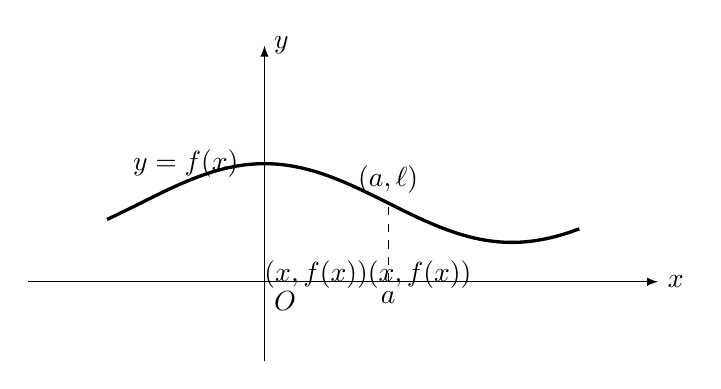
\begin{tikzpicture}[>=latex]
\draw[->](-3,0)--(5,0)node[right]{$x$};  
\draw[->](0,-1)--(0,3)node[right]{$y$};    
\draw[domain=-2:4, samples=100, very thick]plot(\x, {.5*cos(\x r)+1});
\node at (0,0)[below right]{$O$};
\node at (-1,1.5){$y=f(x)$};
\draw[dashed](pi/2,0)node[below]{$a$}--(pi/2,1)node[above]{$(a,\ell)$};

\tkzDefPoints{1.57/1/A, 1.3/1.133/B, 1.8/0.886/C}
\tkzDrawPoints(A,B,C)
\tkzLabelPoint[below left](B){$(x,f(x))$}
\tkzLabelPoint[above right](C){$(x,f(x))$}
\end{tikzpicture}
    \caption{}
\end{figure}

初学的人常常要问:为什么在定义中谈到$x$趋近于$a$时,要限制$x$始终不等于$a$呢?这是因为我们关心的是函数$f(x)$在$a$附近的变化趋势,它和函数$f(x)$在
$x=a$这一点的值没有什么必然关系,这也就是说,无论$f(x)$在点$a$取什么值甚至没有定义,都不影响在这一点的极限的存在和极限值.

\begin{example}
设$f(x)=\frac{3}{4}\cdot \frac{x^2-1}{x-1}$,$x\in(-\infty,1)\cup(1,+\infty)$,求$\Lim_{x\to 1}f(x)$
\end{example}

\begin{solution}
    $f(x)=\frac{3}{4}\cdot \frac{x^2-1}{x-1}$在$x=1$时无意义,因为那时
    分母就变成零,因此,这里没有函数值$f(1)$, 曲线$y=f(x)$也没有相应于横坐标为1的那个点,但是让$x$任意地趋近于1是完全可以的,若$x\ne 1$, 则有
  \[  f (x) =\frac{3}{4}\cdot  \frac{(x-1)(x+1)}{x-1}=\frac{3}{4}(x+1)\]
  因此,不论$x$通过怎样一个以1为极限的数列$\{x_n\}$, 对于相应的数列$\{f(x_n)\}$, 我们都有
  \[\lim_{x_n\to 1} f (x_n) =\frac{3}{4} (1+1) =\frac{3}{2}\]

    从几何上看,曲线$y=f(x)$除去点$\left(1,1\frac{1}{2}\right)$外是与直线$y=\frac{3}{4}(x+1)$一致的,唯独在那一点,曲线有个空隙,而在$x=1$的邻近的点只要充分接近于点1, 所对应的函数值与$\frac{3}{2}$的差的绝对值可以任意小,如图1.3.
\end{solution}
    
\begin{figure}[htp]
    \centering
\begin{tikzpicture}[>=latex]
    \draw[->](-3,0)--(5,0)node[right]{$x$};
    \draw[->](0,-1.5)--(0,4.5)node[right]{$y$};
\foreach \x in {1,2,3}
{
    \draw(0,\x)node[left]{$\x$}--(.1,\x);
    \draw(\x,0)node[below]{$\x$}--(\x,.1);
}
\node at (.25,-.25){$O$};
\draw[dashed](0,1.5)--(1,1.5)--(1,0);
\draw[domain=-2:4, samples=10, very thick]plot(\x, {0.75*(\x+1)});
\draw(1,1.5)[fill=white]  circle(1.5pt) node[right]{$\left(1,1\tfrac{1}{2}\right)$};
\node at (3.25,3)[right]{$y=\frac{3}{4}\cdot \frac{x^2-1}{x-1}$};
\end{tikzpicture}
    \caption{}
\end{figure}

\begin{example}
证明当$x\to 0$时,函数$f(x)=\sin\frac{1}{x}$没有极限.
\end{example}

\begin{proof}
函数$f(x)=\sin\frac{1}{x}$对于一切$x\ne 0$的值有定义,因此这个函数在点$x=0$的领域内有定义.

当$x$取数列$\{x_n\}=\left\{\frac{2}{(2n+1)\pi}\Big| n=1,2,3,\ldots\right\}$的值而趋于零时,数列$\left\{\frac{1}{x_n}\right\}$相应的值是
\[\frac{3\pi}{2},\frac{5\pi}{2},\frac{7\pi}{2},\ldots,(2n+1)\frac{\pi}{2},\ldots\]
此时数列$\left\{\sin\frac{1}{x_n}\right\}$便交替地取$-1$和$+1$这两个数值,换言之
\[\sin\frac{1}{x_n}=(-1)^n,\qquad n=1,2,3,\ldots\]
因此,当$n\to\infty$时,数列$\left\{\sin\frac{1}{x_n}\right\}$不趋于任何极限值.这就证明了当$x\to 0$时,函数$f(x)=\sin\frac{1}{x}$的极限不存在.
\end{proof}

函数的图象大致如图1.4所示.曲线关于原点对称,在包含原点的每一个对称邻域$(-\delta, \delta)$内,曲线$y=\sin\frac{1}{x}$
在原点的邻近作无数次振动,且曲线的振幅恒为1, 虽将原点的邻域的长缩小,也不能减少振动的次数.

\begin{figure}[htp]
    \centering
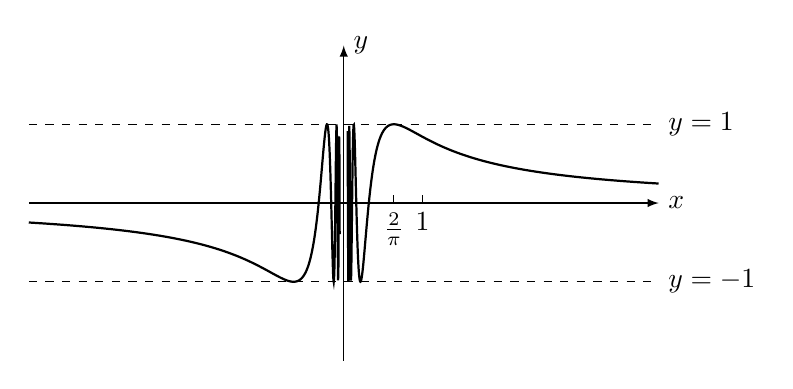
\begin{tikzpicture}[>=latex]
    \draw[->](-4,0)--(4,0)node[right]{$x$};
    \draw[->](0,-2)--(0,2)node[right]{$y$};
    \foreach \x in {1,-1}
    {
        \draw[dashed](-4,\x)--(4,\x)node[right]{$y=\x$};
    }
\draw[domain=-4:-.05, samples=1000, thick]plot(\x, {sin(180/pi/\x)});
\draw[domain=.05:4, samples=1000, thick]plot(\x, {sin(180/pi/\x)});
\foreach \x/\xtext in {1/1, .637/\frac{2}{\pi}}
{
    \draw(\x, 0)node[below]{$\xtext$}--(\x,.1);
}
\end{tikzpicture}    
    \caption{}
\end{figure}

上面是用数列的极限来说明函数的极限,其实我们也可以直接定义函数极限.

\begin{blk}{定义3}
  如果函数$f$在点$a$邻域上有定义(可能去掉点$a$本身),使得当$0<|x-a|<\delta$时,就有$|f(x)-\ell|<\varepsilon$, 那么就说$\ell$为当$x$趋近于$a$时,函数$f$在点$a$的极限值.
\end{blk}

我们对这个定义需要说明以下几点:
\begin{enumerate}
    \item 用定义3验证某数$\ell$是函数$f$在点$a$的极限的办法就是对于任给的$\varepsilon>0$, 要找到这样的正数$\delta$使得能够由不等式$|x-a|<\delta$推出不等式$|f(x)-\ell|<\varepsilon$,虽然$\varepsilon$是任意的正数,但是在找$\delta$的过程中,$\varepsilon$是固定不变的,$\delta$依赖于$\varepsilon$.
    \item 对于已给的$\varepsilon$, 只要证明有一个$\delta>0$存在就行.因为如果有一个$\delta$存在,把$\delta$再缩小一些,显然仍满足我们的要求.
    \item 不等式$|x-a|>0$只是说明$x\ne a$, 即把$x$等于$a$的情况去掉,这是因为我们关心的是函数$f$在点$a$附近的变化趋势,而和函数在$x=a$这点的值无关.
    \item 我们指出定义2和定义3是等价的.
\end{enumerate}

\begin{example}
用定义3证明$\Lim_{x\to 1}\frac{x^3-1}{x-1}=3$
\end{example}

\begin{proof}
    任给$\varepsilon>0$, 要找$\delta>0$, 使由$0<|x-1|<\delta$推出
    $\left|\frac{x^3-1}{x-1}-3\right|<\varepsilon$成立.

    当$x\ne 1$时,
\[\begin{split}
    \left|\frac{x^3-1}{x-1}-3\right|&=|(x^2+x+1)-3|\\
    &=|(x-1)(x+2)|=|x-1|\cdot |x-2|
\end{split}\]

要由$|x-1|\cdot |x+2|<\varepsilon$找$\delta$,显然,这里因子$|x+2|$引起了麻烦.为方便起见,先假定$0<|x-1|<1$,即取$\delta_1=1$,这样
\[0<|x-1|<1\quad\to \quad |x+2|=|(x-1)+3|\le |x-1|+3<4\]因此,要使
\[\begin{cases}
    0<|x-1|<1\\
    |x-1|\cdot |x+2|<\varepsilon
\end{cases}\]
只须
\[\begin{cases}
    0<|x-1|<1\\
    4|x-1|<\varepsilon
\end{cases}\to \quad \begin{cases}
    0<|x-1|<1\\
    |x-1|<\frac{\varepsilon}{4}
\end{cases}\]
由此可见,只须取$\delta=\min\left(1,\frac{\varepsilon}{4}\right)$,即取$\delta$为1与$\frac{\varepsilon}{4}$中的较小者.

$\therefore\quad $对于任意$\varepsilon>0$,取$\delta=\min\left(1,\frac{\varepsilon}{4}\right)$,则当$0<|x-1|<\delta$时,即有
\[\left|\frac{x^3-1}{x-1}-3\right|<\varepsilon\]
这也就证明了
\[\lim_{x\to 1}\frac{x^3-1}{x-1}=3\]
\end{proof}

\begin{example}
    证明$\Lim_{x\to a}\sqrt{x}=\sqrt{a}\quad (a>0)$
\end{example}

\begin{proof}
对于任意的$\varepsilon>0$, 我们必须找到一个$\delta>0$, 使得当$|x-a|<\delta$时,$|\sqrt{x}-\sqrt{a}|<\varepsilon$成立,因为
\[|\sqrt{x}-\sqrt{a}|=\frac{|x-a|}{\sqrt{x}+\sqrt{a}}<\frac{|x-a|}{\sqrt{a}}\]
所以要使$\frac{|x-a|}{\sqrt{a}}<\varepsilon$,只须$|x-a|<\sqrt{a}\varepsilon$

如果取$\delta=\sqrt{a}\varepsilon$,则$\frac{|x-a|}{\sqrt{a}}<\frac{\sqrt{a}\varepsilon}{\sqrt{a}}=\varepsilon$
因此,对于任意$\varepsilon>0$,取$\delta=\sqrt{a}\varepsilon$,则当$|x-a|<\delta$时,就有$|\sqrt{x}-\sqrt{a}|<\varepsilon$成立.这也就证明了
\[\lim_{x\to a}\sqrt{x}=\sqrt{a}\quad (a>0)\]
\end{proof}

有时虽然$f(x)$在某点的左边(或右边)没有定义,如图1.5中的$a,b$两点,我们也可以谈论$f$在点$a$或点$b$两点的极限,譬如对于所有小于$a$的数,$f$虽然没有定义,但是我们可以考察,当$x$从$a$的右侧趋近于$a$时,函数$f$的变化趋势,也就是考察$f$的单边极限是否存在.

\begin{figure}[htp]
    \centering
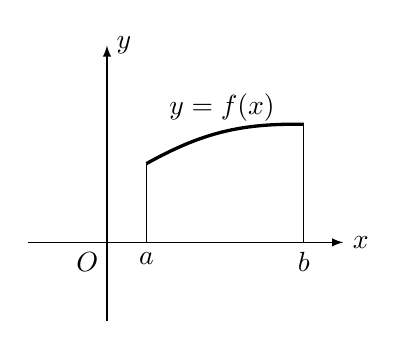
\begin{tikzpicture}[>=latex]
    \draw[->](-1,0)--(3,0)node[right]{$x$};
    \draw[->](0,-1)--(0,2.5)node[right]{$y$};
\draw[very thick](.5,1)to[bend right=-15]node[above]{$y=f(x)$} (2.5,1.5);
\draw(.5,1)--(.5,0)node[below]{$a$};
\draw(2.5,1.5)--(2.5,0)node[below]{$b$};
\node at (-.25,-.25){$O$};
\end{tikzpicture}
    \caption{}
\end{figure}

\begin{blk}{定义}
     设$f(x)$在区间$(a,b)$上有意义,如果任给$\varepsilon>0$, 总存在某个$\delta>0$使得当$x\in (a,a+\delta)$时,总有$|f(x)-\ell|<\varepsilon$,我们就说函数$f$在点$a$以$\ell$为\textbf{右极限},记作:
\[\lim_{x\to a^+}f(x)=\ell\]
\end{blk}

类似地,可以定义\textbf{左极限},只需把开区间$(a,a+\delta)$换成$(b-\delta,b)$就行了,并记作
\[\lim_{x\to b^-} f(x)=\ell\]

\begin{example}
    设函数$f(x)=\begin{cases}
        x-1,&x\le 1\\
x+1,&x>1
    \end{cases}\quad $    
    求$\Lim_{x\to 1^-}f(x)$和$\Lim_{x\to 1^+}f(x)$
\end{example}

\begin{figure}[htp]
    \centering
    \begin{minipage}[t]{0.48\textwidth}
    \centering
    \begin{tikzpicture}[>=stealth, scale=.6]
        \draw[->](-3,0)--(4,0)node[right]{$x$};
        \draw[->](0,-3)--(0,4.5)node[right]{$y$};
        \draw(0,1)node[left]{1}--(.1,1);
        \draw(0,2)node[left]{2}--(.1,2);
        \draw(1,0)node[below]{1}--(1,.1);
        \node at (-.25,-.25){$O$};
        \draw[domain=-2:1, samples=10, very thick]plot(\x,{\x-1});
        \draw[domain=1:3, samples=10, very thick]plot(\x,{\x+1});
    \node at (-2,-3)[left]{$y=x-1$};
    \node at (3,4)[right]{$y=x+1$};
    \draw[dashed](1,0)--(1,2)--(0,2);
    \draw (1,2)[fill=white] circle(2.5pt);
    
    \end{tikzpicture}
    \caption{}
    \end{minipage}
    \begin{minipage}[t]{0.48\textwidth}
    \centering
    \begin{tikzpicture}[>=stealth, scale=.8]
        \draw[->](-3,0)--(4,0)node[right]{$x$};
    \draw[->](0,-2.5)--(0,3)node[right]{$y$};
    \foreach \x in {-2,-1,1,2,3}
    {
        \draw(\x,0)node[below]{$\x$}--(\x,.1);
    }
\foreach \x in {-2,-1,1,2}
{
    \draw(0,\x)--(.1,\x)node[right]{$\x$};
}
\foreach \x in {-2,-1,...,2}
{
    \draw[very thick](\x,\x)--(\x+1,\x);
    \draw (\x+1,\x)[fill=white]circle(2pt);
}
    \node at (.25,-.25){$O$};
    \end{tikzpicture}
    \caption{}
    \end{minipage}
    \end{figure}


\begin{solution}
\[\begin{split}
    \lim_{x\to 1^-}f(x)&=\lim_{x\to 1^-}(x-1)=0\\
    \lim_{x\to 1^+}f(x)&=\lim_{x\to 1^+}(x+1)=2
\end{split}\]
图1.6显示了上面的结果.
\end{solution}

\begin{example}
    函数$y=[x]$代表不超过$x$的最大整数,即若$n\le x<n+1$,$n\in\mathbb{Z}$,则$y=[x]=n$.(图1.7)

求$\Lim_{x\to 2^+}\frac{[x]}{x},\quad \Lim_{x\to 2^-}\frac{[x]}{x}$
\end{example}

\begin{solution}
    显然,当$x=2$时,$\frac{[x]}{x}=\frac{[2]}{2}=\frac{2}{2}=1$, 又
\[\frac{[x]}{x}=\begin{cases}
    \frac{1}{x},& x\in(1,2)\\
    \frac{2}{x},& x\in(2,3)
\end{cases}\]
所以
\[\begin{split}
    \lim_{x\to 2^+}\frac{[x]}{x}&=\lim_{x\to 2^+}\frac{2}{x}=1\\
     \lim_{x\to 2^-}\frac{[x]}{x}&=\lim_{x\to 2^-}\frac{1}{x}=\frac{1}{2}
\end{split}\]    
\end{solution}


下面的命题说明函数的极限与函数的单边极限的关系:

\begin{blk}{定理}
极限$\Lim_{x\to a} f(x)$
存在的必要和充分条件是左极限$\Lim_{x\to a^-} f(x)$和右极限$\Lim_{x\to a^+} f(x)$都存在,并且二者相等.
\end{blk}

\begin{proof}
    必要性
    
    如果$\Lim_{x\to a} f(x)=\ell$, 就是说任给$\varepsilon>0$, 总存在$\delta>0$,
使得当$0<|x-a|<\delta$, 即当$x\in (a-\delta,a)\cup(a,a+\delta)$时,有$|f(x)-\ell|<\varepsilon$.换言之,当$x\in (a-\delta,a)$和$x\in (a,a+\delta)$时,都有$|f (x) -\ell|<\varepsilon$,因此
\[\Lim_{x\to a^-} f(x)=\ell,\qquad \Lim_{x\to a^+} f(x)=\ell\]

充分性

如果$\Lim_{x\to a^-} f(x)=\ell$且$\Lim_{x\to a^+} f(x)=\ell$, 那么总存在$\delta_1>0$, 使得当$x\in(a-\delta_1,a)$时,有
$|f (x) -\ell|<\varepsilon$.

又存在$\delta_2>0$, 使得当$x\in (a,a+\delta_2)$时,有$|f (x) -\ell|<\varepsilon$.

取$\delta=\min(\delta_1,\delta_2)$,于是当$x\in(a-\delta,a+\delta)$时,有$|f (x) -\ell|<\varepsilon$.
这就是说:
\[\Lim_{x\to a} f(x)=\ell\]
\end{proof}

\begin{example}
说明$\Lim_{x\to 3}\frac{|x-3|}{x-3}$是否存在?
\end{example}

\begin{solution}
\[\begin{split}|x-3|&=\begin{cases}
    x-3, & x>3\\
    3-x, &x<3
\end{cases}\\
    \Lim_{x\to 3^-}\frac{|x-3|}{x-3}&=\Lim_{x\to 3^-}\frac{3-x}{x-3}=\Lim_{x\to 3^-}(-1)=-1\\
    \Lim_{x\to 3^+}\frac{|x-3|}{x-3}&=\Lim_{x\to 3^+}\frac{x-3}{x-3}=\Lim_{x\to 3^+}(1)=1
\end{split}\]

$\because\quad \Lim_{x\to 3^-}\frac{|x-3|}{x-3}\ne \Lim_{x\to 3^+}\frac{|x-3|}{x-3}$
    
$\therefore\quad \Lim_{x\to 3}\frac{|x-3|}{x-3}$
不存在.
\end{solution}

\subsection{函数值趋于无穷大}

如果函数$f$在点$a$的邻域上有定义(可能去掉点$a$本身)对于无论多么大的正数$G$, 总存在一个够小的正数$\delta$, 使得当$0<|x-a|<\delta$时,就有$|f(x)|>G$, 那么就说当$x$趋于$a$时,函数$f(x)$趋于\textbf{无穷大},记作
\[\lim_{x\to a} f (x) =\infty\]

\begin{example}
    求证$\Lim_{x\to 0}\frac{1}{x}=\infty$
\end{example}
   
\begin{proof}
设$G$是任意给定的正数,我们要求出一个$\delta>0$, 使得当$|x|<\delta$时,$|f(x)|=\left|\frac{1}{x}\right|>G$.

事实上,要使$\frac{1}{|x|}>G$, 
只须$0<|x|<\frac{1}{G} $.取$\delta=\frac{1}{G}$, 于是当$|x|<\delta$时,就有$\frac{1}{|x|}>G$
因此,
$$\Lim_{x\to 0}\frac{1}{x}=\infty$$
\end{proof}

\begin{example}
    证明当$x\to 0$时,函数$f(x)=\frac{1}{x}\sin\frac{1}{x}\quad (x\ne 0)$不趋于无穷大.
\end{example}

\begin{proof}
如果自变量$x$取数列$\{x_n\}=\left\{\frac{2}{(2n+1)\pi}\Big|n=1, 2, 3,\ldots\right\}$的值趋于0时,$\sin\frac{1}{x}$在原点的任意邻域内无限次交替地取$-1, 1$这两个值,对于这些值,$|f(x)|=\frac{1}{x}=\frac{\pi}{2}(2n+1)$趋于无穷大.

但是当$x$取数列$\{x\}=\left\{\frac{1}{n\pi}\Big| n=1, 2, 3,\ldots\right\}$的
值趋于0时,由于
$\sin\frac{1}{x}=\sin (n\pi) =0$, 
故对于这些值,
$\Lim_{x'_n\to 0} f (x) =0$.

可见在原点的邻近不存在这样的$\delta>0$, 使得当$|x|<\delta$时,$|f(x)|>G$, 因此,当$x\to 0$时,$f(x)=\frac{1}{x}\sin\frac{1}{x}\quad (x\ne 0)$不趋于无穷大.

$y=f(x)$的图象位于两条双曲线$xy=\pm 1$之间,且在原点的邻近作无限多次振动,越靠近原点,曲线的振幅越大(图1.8).

\begin{figure}[htp]
    \centering
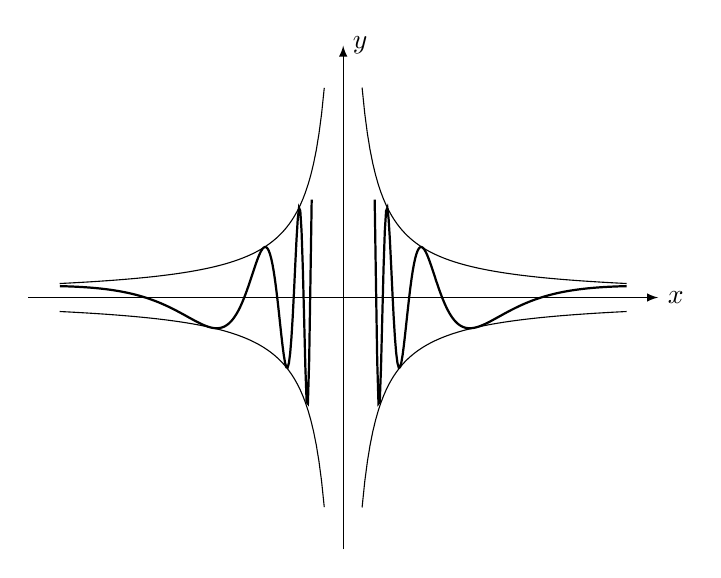
\begin{tikzpicture}[>=latex, scale=.8]
\draw[->](-5,0)--(5,0)node[right]{$x$};
\draw[->](0,-4)--(0,4)node[right]{$y$};
\draw[domain=-4.5:-.3, samples=100]plot(\x,{-1/\x}); 
\draw[domain=-4.5:-.3, samples=100]plot(\x,{1/\x}); 
\draw[domain=.3:4.5, samples=100]plot(\x,{-1/\x}); 
\draw[domain=.3:4.5, samples=100]plot(\x,{1/\x}); 
\draw [domain=.5:4.5, samples=200,  thick]plot(\x, {sin(180/\x*pi)/\x});
\draw [domain=.5:4.5, samples=200,  thick]plot(-\x, {sin(180/\x*pi)/\x});
\end{tikzpicture}
    \caption{}
\end{figure}

\end{proof}

如果对于任何$G>0$, 存在$\delta>0$, 当$0<|x-a|<\delta$时,有$f(x)>G$, 就说当$x\to a$时,函数$f(x)$趋于正无无穷大,记作
\[\lim_{x\to a}f(x)=+\infty\]

如果对于任何$G>0$, 存在$\delta>0$, 当$0<|x-a|<\delta$时,有$f(x)<-G$, 就说当$x\to a$时,函数$f(x)$趋于负无穷大,记作
\[\lim_{x\to a}f(x)=-\infty\]

例如,我们有:
\[\lim_{x\to 0}\frac{1}{x^2}=+\infty,\qquad \lim_{x\to 0}\frac{(-1)}{x^2}=-\infty\]

类似地,我们可以定义:
\[\lim_{x\to a^-}f(x)=+\infty,\quad \lim_{x\to a^+}f(x)=+\infty,\quad \lim_{x\to a^-}f(x)=-\infty,\quad \lim_{x\to a^+}f(x)=-\infty\]
的含义,这里不再写出.建议读者将这些定义严格地写出来.

例如,我们有:
\[\lim_{\theta\to \tfrac{\pi^+}{2}}\tan\theta =+\infty,\qquad \lim_{\theta\to \tfrac{\pi^-}{2}}\tan\theta =-\infty\]
\[\lim_{x\to 0^+}\log_a x =-\infty\quad (a>1),\qquad \lim_{x\to 0^+}\log_a x =+\infty\quad (0<a<1)\]

\begin{ex}
\begin{enumerate}
    \item 用函数极限定义证明:
    \begin{multicols}{2}
        \begin{enumerate}
            \item $\Lim_{x\to \infty}\frac{1}{2x+1}=0$
            \item $\Lim_{x\to 2}x^2=4$
            \item $\Lim_{x\to -1}\frac{x-3}{x^2-9}=\frac{1}{2}$
            \item $\Lim_{x\to 1}\frac{1}{x^2}=1$
            \item $\Lim_{x\to 1}\frac{x^3-x}{x-1}=2$
        \end{enumerate}
    \end{multicols}
    \item 说明:$\Lim_{x\to 3}\frac{x}{x^2-9}=\infty$
    \item 下面极限是否存在?
\begin{multicols}{2}
    \begin{enumerate}
        \item $\Lim_{x\to 1}\frac{2x|x-1|}{x-1}$
        \item $\Lim_{x\to 3}\frac{[x]^2-9}{x^2-9}$
    \end{enumerate}
\end{multicols}
\end{enumerate}
\end{ex}

\subsection{函数极限算法定理}
函数的极限算法定理与数列的极限算法定理类似,因为所谓$\Lim_{x\to a}u(x)=A$, $\Lim_{x\to a}v(x)=B$的意思就是对于任何一个各项都不同于$a$并且以$a$为极限的数列$x_n\to a$, 便有函数值数列$\{u(x_n)\}$, $\{v(x_n)\}$, 并且$\Lim_{n\to \infty}u(x_n)=A$, 
$\Lim_{n\to \infty} v(x_n)=B$, 因此,根据第四册下第三章的定理就可以直接得到相应的结果.现在给出函数的极限运算定理如下:

\begin{blk}{定理}
设$\Lim_{x\to a}u(x)=A$, $\Lim_{x\to a}v(x)=B$,那么
\begin{enumerate}
    \item $\Lim_{x\to a}[u(x)+v(x)]=\Lim_{x\to a}u(x)+\Lim_{x\to a}v(x)$
    \item $\Lim_{x\to a}[u(x)\cdot v(x)]=\Lim_{x\to a} u(x)\cdot \Lim_{x\to a}v(x)$
    \item $\Lim_{x\to a}[c\cdot u(x)]=c\cdot \Lim_{x\to a}u(x)$
    \item $\Lim_{x\to a}\frac{u(x)}{v(x)}=\frac{\Lim_{x\to a}u(x)}{\Lim_{x\to a}v(x)}$ 
    
    只要$v(x)$恒不为0,而且$\Lim_{x\to a}v(x)\ne 0$
    \item $\Lim_{x\to a}\sqrt[n]{u(x)}=\sqrt[n]{\Lim_{x\to a}u(x)}$
    \item 如$\Lim_{x\to a}u(x)=A=\Lim_{x\to a} v(x)$,而$|x-a|<\delta$时,$u(x)<f(x)<v(x)$,则:
    \[\Lim_{x\to a} f(x)=A\]
    即:如果$u(x)$与$v(x)$趋向同一极限$A$,且$f(x)$在$u(x)$与$v(x)$之间,那么,$f(x)$便也趋向那个极限$A$.
\end{enumerate}
\end{blk}

现在只有5需要补证.

设$\Lim_{x\to a}u(x)=A>0$, 则根据函数极限定义:对于$\varepsilon=\frac{A}{2}>0$, 存在$\delta>0$,使得$0<|x-a|<\delta$时,有
\begin{equation}
    u(x)>\frac{A}{2}>0
\end{equation}

于是,
\[\sqrt[n]{u(x)}-\sqrt[n]{A}=\frac{u(x)-A}{\sum^n_{k=1}[u(x)]^{\tfrac{n-k}{n}}A^{\tfrac{k-1}{n}}}\]
由(1.3)式
\[[u(x)]^{\tfrac{n-k}{n}}>\left(\frac{A}{2}\right)^{\tfrac{n-k}{n}}\]
故
\[\begin{split}
    \sum^n_{k=1}[u(x)]^{\tfrac{n-k}{n}}A^{\tfrac{k-1}{n}}&>\sum^n_{k=1}\left(\frac{A}{2}\right)^{\tfrac{n-k}{n}}A^{\tfrac{k-1}{n}}\\
    &=A^{\tfrac{n-1}{n}}\sum^n_{k=1}\left(\frac{1}{2}\right)^{\tfrac{n-k}{n}}\\
    &=A^{\tfrac{n-1}{n}}\left\{\left(\frac{1}{2}\right)^{\tfrac{n-1}{n}}+\left(\frac{1}{2}\right)^{\tfrac{n-2}{n}}+\cdots+\left(\frac{1}{2}\right)^{\tfrac{1}{n}}+1\right\}\\
    &=A^{\tfrac{n-1}{n}}\left\{\frac{1-\left(\frac{1}{2}\right)^{\tfrac{n-1}{n}}\cdot \left(\frac{1}{2}\right)^{\tfrac{1}{n}}}{1-\left(\frac{1}{2}\right)^{\tfrac{1}{n}}}\right\}\\
    &=A^{\tfrac{n-1}{n}}\cdot\frac{\frac{1}{2}}{1-\left(\frac{1}{2}\right)^{\tfrac{1}{n}}}=\frac{A^{\tfrac{n-1}{n}}}{2-2^{\tfrac{n-1}{n}}}\\
\end{split}\]
$\therefore\quad \left|\sqrt[n]{u(x)}-\sqrt[n]{A}\right|<|u(x)-A|\cdot \frac{2-2^{\tfrac{n-1}{n}}}{A^{\tfrac{n-1}{n}}}$

由题设$\Lim_{x\to a}u(x)=A$,而$\frac{2-2^{\tfrac{n-1}{n}}}{A^{\tfrac{n-1}{n}}}$是一个与$x$无关的常数,所以
\[\lim_{x\to a} \sqrt[n]{u(x)}=\sqrt[n]{A}=\sqrt[n]{\lim_{x\to a}u(x)}\]

下面我们来证明两个重要极限公式,为此先介绍一个引理.

\begin{blk}{引理}
     对于任意实数$\theta$, 都有$|\sin\theta|\le |\theta|$
\end{blk}

\begin{proof}
  由于对于任意实数.有$|\sin\theta|\le 1$, 那么仅考虑$\theta\in (0,\pi/2)$即可.
  
  在单位圆$O$上(图1.9),
 截取弧$\wideparen{P_0M}$使弧长$|\wideparen{P_0M}|$等于$\theta$, 其中$P_0$和$M$分别有坐标$(1, 0)$和$(x,y)$, 于是
 \[\sin\theta =y<\sqrt{y^2+ (1-x)^2} =|P_0M|<|\wideparen{P_0M}|=\theta\]
 
 显然,当$\theta=0$时,有$\sin\theta=\theta$. 因此
\[  |\sin\theta | \le |\theta|,\qquad  \theta\in  (0,\pi/2)\]

  如果$-\pi/2<\theta<0$, 则仍有$|MN|<\wideparen{P_0M}$,于是
\[|\sin\theta|<|\theta|,\qquad \theta\in (-\pi/2, 0) \]

  如果$|\theta|\ge \pi/2$, 则因为$\pi/2>1$与$|\sin\theta|\le 1$, 而同样地也得到$|\sin\theta|<|\theta|$. 
  
  因此,对于一切$\theta\ne 0$的值,有$|\sin\theta|<|\theta|$; 当$\theta=0$时,有$|\sin\theta|=|\theta|$.
\end{proof}



\begin{figure}[htp]\centering
    \begin{minipage}[t]{0.48\textwidth}
    \centering
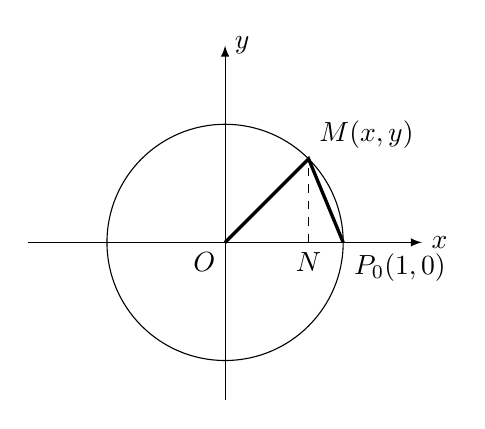
\begin{tikzpicture}[>=latex]
\draw[->](-2.5,0)--(2.5,0)node[right]{$x$};
\draw[->](0,-2)--(0,2.5)node[right]{$y$};
\draw(0,0) circle(1.5);
\draw[very thick](0,0)--(45:1.5)node[above right]{$M(x,y)$}--(1.5,0)node[below right]{$P_0(1,0)$};
\draw[dashed](1.5/1.414,0)node[below]{$N$}--(1.5/1.414,1.5/1.414);
\node at (0,0)[below left]{$O$};
\end{tikzpicture}    
    \caption{}
    \end{minipage}
    \begin{minipage}[t]{0.48\textwidth}
    \centering
    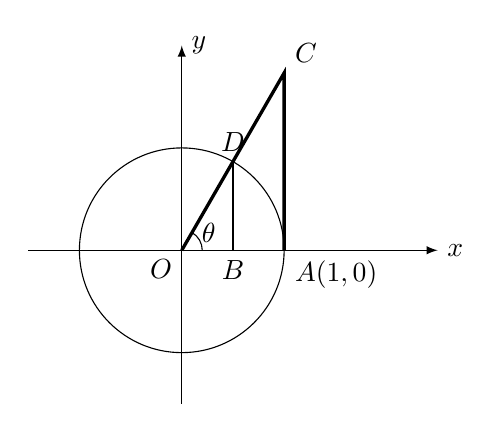
\begin{tikzpicture}[>=latex, scale=1.3]

\draw[->](-1.5,0)--(2.5,0)node[right]{$x$};
\draw[->](0,-1.5)--(0,2)node[right]{$y$};
\draw(0,0) circle(1);
\draw[very thick](0,0)--(60:2)node[above right]{$C$}--(1,0)node[below right]{$A(1,0)$};
\draw[thick](.5,0)node[below]{$B$}--(60:1)node[above]{$D$};
\node at (0,0)[below left]{$O$};   
\draw(0.2,0) arc (0:60:.2)node[right]{$\theta$};   
    \end{tikzpicture}
    \caption{}
    \end{minipage}
    \end{figure}

\begin{blk}{定理}
\[\lim_{\theta\to 0}\frac{\sin\theta }{\theta}=1,\qquad \lim_{\theta\to 0}\frac{\cos\theta-1}{\theta}=0\]
\end{blk}

\begin{proof}
    让我们先证明$\Lim_{\theta\to 0}\frac{\sin\theta }{\theta}=1$.由图1.10容易看出:

假定$\theta$的单位是弧度,于是:
\[\begin{split}
    \triangle OBD\text{的面积}&=\frac{1}{2}OB\cdot BD=\frac{1}{2}\cos\theta\cdot \sin\theta\\
    \triangle OAC\text{的面积}&=\frac{1}{2}OA\cdot AC=\frac{1}{2}\cdot 1\cdot \tan\theta\\
    \text{扇形$OAD$的面积}&=\frac{1}{2}OA\cdot \wideparen{AD}=\frac{1}{2}\cdot 1^2\cdot \theta
\end{split}\]

假如角是用180等分平角的“度”作为单位,则扇形面积就是$\frac{1}{2}\cdot 1\cdot \frac{\pi}{100}\theta$.

因为上述扇形是夹在$\triangle OBD$和$\triangle OAC$之间,所以
\begin{equation}
    \frac{1}{2}\cos\theta\sin\theta<\frac{1}{2}\theta<\frac{1}{2}\tan\theta=\frac{1}{2}\frac{\sin\theta}{\cos\theta}
\end{equation}
即有,若$0<\theta<\frac{\pi}{2}$,则
\begin{equation}
    \cos\theta<\frac{\sin\theta}{\theta}<\frac{1}{\cos\theta}
\end{equation}
注意到:$\sin(-\theta)=-\sin\theta$和$\cos(-\theta)=\cos\theta$, 不等式(1.5)也蕴含,若$-\frac{\pi}{2}<\theta<0$, 则
\begin{equation}
    \cos(-\theta)<\frac{\sin(-\theta)}{-\theta}<\frac{1}{\cos(-\theta)}
\end{equation}
将不等式(1.5)和(1.6)合并为,若$0<|\theta|<\frac{\pi}{2}$,则
\begin{equation}
    \cos\theta<\frac{\sin\theta}{\theta}<\frac{1}{\cos\theta}
\end{equation}
又因为
\[0\le |1-\cos\theta|=\left|2\sin^2\frac{\theta}{2}\right|\le 2\left|\sin\frac{\theta}{2}\right|<|\theta|\]
从而
\[0\le \lim_{\theta\to 0}|1-\cos\theta|\le \lim_{\theta\to 0}|\theta|=0\]
所以
\[\lim_{\theta\to 0}|1-\cos\theta|=0\]
即:$\Lim_{\theta\to 0}\cos\theta=1$
由(1.7)知被夹逼在两者之间的$\frac{\sin\theta}{\theta}$极限值也就一定是1了!

以$\Lim_{\theta\to 0}\frac{\sin\theta}{\theta}=1$为基础,则:
\[\begin{split}
\lim_{\theta\to 0}\frac{\cos\theta-1}{\theta}&=\lim_{\theta\to 0}\left\{\frac{-2\left(\sin\frac{\theta}{2}\right)^2}{\theta}\right\}\\
&= \lim_{\theta\to 0}\left(-\sin\frac{\theta}{2}\right)\frac{\sin\frac{\theta}{2}}{\frac{\theta}{2}}    \\
&=\lim_{\theta\to 0}\left(-\sin\frac{\theta}{2}\right)\cdot \lim_{\theta\to 0}\frac{\sin\frac{\theta}{2}}{\frac{\theta}{2}}   \\
&=0\cdot 1=0
\end{split}   
\]
\end{proof}

\begin{example}
求:$\Lim_{x\to 2}\frac{x^2+3x-10}{3x^2-5x-2},\qquad \Lim_{x\to 0}\frac{\sqrt[3]{1+x^2}-1}{x^2}$
\end{example}

\begin{solution}
    如果应用前面的定理去分别求两式中的分子、分母的极限时,其分子、分母的极限值均为零,即我们得到$\frac{0}{0}$的不定形式.我们通常要对原代数式变形,找出分子、分母中具有$x-a$的因子,消去$x-a$的公共因子,一般问题就可解决.
\[\begin{split}
    \Lim_{x\to 2}\frac{x^2+3x-10}{3x^2-5x-2}&=\Lim_{x\to 2}\frac{(x+5)(x-2)}{(3x+1)(x-2)}\\
    &=\Lim_{x\to 2}\frac{x+5}{3x+1}\\
    &=\frac{2+5}{3\x 2+1}=1
\end{split}\]

\[\begin{split}
    \Lim_{x\to 0}\frac{\sqrt[3]{1+x^2}-1}{x^2}&=\Lim_{x\to 0}\frac{{(1+x^2)}-1}{x^2\left(\sqrt[3]{(1+x^2)^2}+\sqrt[3]{1+x^2}+1\right)}\\
    &=\Lim_{x\to 0}\frac{1}{\sqrt[3]{(1+x^2)^2}+\sqrt[3]{1+x^2}+1}=\frac{1}{3}
\end{split}\]
\end{solution}

\begin{example}
    求:$\Lim_{x\to 0}\frac{\cos x-1}{x^2},\qquad \Lim_{x\to \pi}\frac{\sin mx}{\sin nx}(m,n\in \mathbb{N})$
\end{example}

\begin{solution}
\[\begin{split}
    \Lim_{x\to 0}\frac{\cos x-1}{x^2}&=\Lim_{x\to 0}\frac{-2\left(\sin\frac{x}{2}\right)^2}{x^2}\\
    &=\frac{-2}{2^2}\Lim_{x\to 0}\frac{\sin\frac{x}{2}}{\frac{x}{2}}\cdot \Lim_{x\to 0}\frac{\sin\frac{x}{2}}{\frac{x}{2}}\\
    &=\left(-\frac{1}{2}\right)\cdot 1\cdot 1=-\frac{1}{2}
\end{split}\]

由三角函数诱导公式易知
\[\sin m(\pi-x)=\sin(m\pi-mx)=(-1)^{m-1}\sin mx\]
同样得到
\[\sin n(\pi-x)=(-1)^{n-1}\sin nx\]
因此:
\[(-1)^{m-n}\frac{\sin mx}{\sin nx}=\frac{\sin m(\pi-x)}{\sin n(\pi-x)}\]
两边乘以$(-1)^{m-n}$,得
\[\frac{\sin mx}{\sin nx}=(-1)^{m-n}\frac{\sin m(\pi-x)}{\sin n(\pi-x)}\]
设$y=\pi-x$, 则当$x\to \pi$, 有$y\to 0$, $my\to 0$, $ny\to 0$. 因此:
\[\begin{split}
    \Lim_{x\to \pi}\frac{\sin mx}{\sin nx}&=\lim_{y\to 0}(-1)^{m-n}\frac{\sin my}{\sin ny}\\
&=(-1)^{m-n}\lim_{y\to 0}\left(\frac{m}{n}\cdot \frac{\sin my}{my}\cdot \frac{ny}{\sin ny}\right)\\
&=(-1)^{m-n}\cdot \frac{m}{n}\cdot 1\cdot 1=(-1)^{m-n}\frac{m}{n}
\end{split}\]
\end{solution}

\begin{example}
由条件$\Lim_{x\to -\infty}\left(\sqrt[]{x^2-x+1}-ax-b\right)=0$,求出$a,b$的值.
\end{example}

\begin{solution}
$\because\quad \Lim_{x\to -\infty}\left(\sqrt{x^2-x+1}-ax-b\right)=0,\quad \Lim_{x\to -\infty}\frac{1}{x}=0$

$\therefore\quad \Lim_{x\to -\infty}\left(\sqrt{x^2-x+1}-ax-b\right)\cdot \frac{1}{x}=0$

即:
\[\Lim_{x\to -\infty}\left(\frac{\sqrt{x^2-x+1}}{x}-a-\frac{b}{x}\right)=0\]
又因为:当$x<0$时,
\[\sqrt{x^2-x+1}=\sqrt{x^2\left(1-\frac{1}{x}+\frac{1}{x^2}\right)}=-x\sqrt{1-\frac{1}{x}+\frac{1}{x^2}}\]
所以上式可写成
\[\lim_{x\to -\infty}\left(-\sqrt{1-\frac{1}{x}+\frac{1}{x^2}}-a-\frac{b}{x}\right)=0\]
即:$-1-a-0=0\quad \to \quad a=-1$

代入原条件,得
\[\lim_{x\to -\infty}\left(\sqrt{x^2-x+1}+x-b\right)=0\]
即:
\[\begin{split}
    b&=\lim_{x\to-\infty}\left(\sqrt{x^2-x+1}+x\right)\\
    &=\lim_{x\to-\infty} \frac{x^2-x+1-x^2}{\sqrt{x^2-x+1}-x}  \\
    &=\lim_{x\to-\infty}\frac{-x\left(1-\frac{1}{x}\right)}{-x\left(\sqrt{1-\frac{1}{x}+\frac{1}{x^2}}+1\right)}    \\
    &=\lim_{x\to-\infty}\frac{1-\frac{1}{x}}{\sqrt{1-\frac{1}{x}+\frac{1}{x^2}}+1} =\frac{1}{2}   \\
\end{split}\]

$\therefore\quad a=-1,\quad b=\frac{1}{2}$为所求.
\end{solution}

\begin{ex}
\begin{enumerate}
    \item 说明当$x\to \infty$时,函数$\frac{x^5-4}{x^3+x}$的变化趋势.
    \item 求极限
    \begin{enumerate}
\begin{multicols}{2}
    \item  $\Lim _{x \to 0} \frac{(x+2)^{2}}{x^{2}+4}$
    \item  $\Lim _{x \to 2} \frac{x^{2}-4}{x-2}$
    \item  $\Lim _{x \to 2} \frac{5 x^{2}+x-8}{x^{2}-4}$
    \item  $\Lim _{x \to 0} \frac{\left(4 x^{3}-3\right)(1-2 x)}{7 x^{3}-6 x+4}$
    \item  $\Lim _{x \to \infty} \frac{3 x^{5}}{x^{5}-x^{2}+1}$
    \item  $\Lim _{x \to \infty} \frac{\left(x^{2}-5\right)\left(x^{2}+7\right)}{x^{4}+35}$
    \item  $\Lim _{x \to 3} \frac{x^{2}-8 x+15}{x^{2}-7 x+12}$
    \item  $\Lim _{x \to -3} \frac{x^{2}-9}{x^{2}+9 x+18}$
    \item $\Lim _{x \to -1} \frac{x\left(x^{2}+4 x+3\right)}{x^{3}+3 x^{2}+5 x+3}$
    \item  $\Lim _{x \to 1} \frac{x^{3}+x^{2}-2}{x^{4}+2 x^{2}-2 x-1}$
    \item $\Lim _{x \to \infty} \frac{x+\sin x}{2 x+5}$
    \item  $\Lim _{x \to 0} \frac{(1+x)^{5}-(1+5 x)}{x^{2}+x^{5}}$
\end{multicols}
    \item  $\Lim _{x \to 0} \frac{(1+m x)^{n}-(1+n x)^{m}}{x^{2}}\qquad (m, n \in \mathbb{N})$
    \item  $\Lim _{x \to 1} \frac{x^{2}+x^{4}+\cdots+x^{2 n}-n}{x-1}$
\end{enumerate}

    \item 求极限  
\begin{enumerate}
\begin{multicols}{2}
\item $\Lim_{x\to 0^+}\sqrt{3x} $
\item $\Lim_{x\to 1^-}\sqrt{1-x} $
\item $\Lim_{x\to 3^-} 3[x]$
\item $\Lim_{x\to 1^+} [x+3]$
\item $\Lim_{x\to -3^+}\left(1+\sqrt{x+3}\right) $
\item $\Lim_{x\to 4^-} \left(\sqrt{4-x}+[x-1]\right)$
    \item $\Lim_{x\to 1^+}\frac{2x|x-1|}{x-1} $
    \item $\Lim_{x\to 4^-} ([x]-x)$
\end{multicols}
    \item $\Lim_{x\to 0^+}\frac{b}{x}\left[\frac{x}{a}\right] \qquad (a>0,\; b>0)$
    \item $\Lim_{x\to 0^+} \frac{x}{a}\left[\frac{b}{x}\right]\qquad (a>0,\; b>0)$
\end{enumerate}    

    \item 求极限  
\begin{enumerate}
\begin{multicols}{2}
\item $\Lim _{x \to  1} \frac{1-x}{\sqrt{1-x^{2}}}$;
\item  $\Lim _{x \to  1} \frac{1-\sqrt{x}}{1-x}$;
\item  $\Lim _{x \to  1} \frac{(2 x-3)(\sqrt{x}-1)}{2 x^{2}+x-3}$
\item  $\Lim _{x \to  2} \frac{x-2}{\sqrt{x^{2}-2}-\sqrt{2}}$
\item  $\Lim _{t \to +\infty}(\sqrt{1+t}-\sqrt{t})$;
\item  $\Lim _{x \to +\infty} \sqrt{x}(\sqrt{x+a}-\sqrt{x})$
\item  $\Lim _{x \to  5} \frac{\sqrt{x-1}-2}{x-5}$;
\item $\Lim _{x \to  0} \frac{\sqrt[3]{1+x}-\sqrt[3]{1-x}}{x}$
\item  $\Lim _{x \to  1} \frac{4 x+\sqrt{x-1}}{2 x-\sqrt{x+1}}$
\item  $\Lim _{x \to  1} \frac{x-1}{\sqrt{x^{2}-1}+\sqrt{x-1}}$
\item $\Lim _{x \to  a} \frac{\sqrt{x-a}+\sqrt{x}-\sqrt{a}}{\sqrt{x^{2}-a^{2}}}$
\item  $\Lim _{x \to -\infty} \frac{x-2}{\sqrt{x^{2}-4 x+3}}$
\item $\Lim _{x \to -\infty}\left[\frac{2(x-1)^{2}}{\sqrt{4 x^{2}+2 x+1}}+x\right]$
\end{multicols}
\item $\Lim _{x \to +\infty}\left(\sqrt{x+\sqrt{x+\sqrt{x}}}-\sqrt{x}\right)$
\item $\Lim _{x \to +\infty} x\left(\sqrt{x^{2}+2 x}-2 \sqrt{x^{2}+x}+x\right)$
\end{enumerate}   

\item \begin{enumerate}
    \item $f(x)=\begin{cases}
        0,& x>1\\
        1,& x=1\\
        x^2+2, &x<1
    \end{cases}$

    求$f(x)$在$x=1$的左右极限.

    \item $f(x)=\begin{cases}
        x\sin\frac{1}{x},& x>0\\
        1+x^2,& x<0
    \end{cases}$

    求$f(x)$在$x=0$的左右极限.

    \item $\Lim_{x\to 3}\frac{[x]^2-9}{x^2-9}$是否存在?
    \item $\Lim_{x\to 0}\frac{x}{|x|}$是否存在?
\end{enumerate}

\item 若$0<x<\frac{\pi}{2}$,求证:
\begin{multicols}{2}
    \begin{enumerate}
        \item $\tan x>x$
        \item $x-\frac{x^2}{4}<\sin x<x$
    \end{enumerate}
\end{multicols}

\item 求极限  
\begin{enumerate}
\begin{multicols}{2}
    \item $\Lim_{x\to 0} \frac{\sin ax}{x}$
    \item $\Lim_{x\to 0} \frac{\sin 7x}{4x}$
    \item $\Lim_{\theta\to 0} \frac{\sec2\theta\sin\theta}{\theta}$
    \item $\Lim_{\theta \to 0} \frac{\tan\theta}{\theta}$
    \item $\Lim_{t\to 0} \frac{15t}{\tan 6t}$
    \item $\Lim_{x\to 0} \frac{\tan 2x}{\sin 7x}$
    \item $\Lim_{\theta \to 0} \frac{\tan\theta-\sin\theta}{\theta^2}$
    \item $\Lim_{x\to 0} \frac{\csc x-\cot x}{x}$
    \item $\Lim_{x\to 0} \frac{\sin^2\frac{x}{2}}{x^2}$
    \item $\Lim_{x\to \pi} \frac{\sin x}{\pi-x}$
    \item $\Lim_{x\to 1} \frac{1+\cos\pi x}{\tan^2 \pi x}$
    \item $\Lim_{x\to \tfrac{\pi}{4}}\tan 2x\tan\left(\frac{\pi}{4}-x\right) $ 
    \item $\Lim_{x\to 1} (1-x)\tan\frac{\pi x}{2}$
    \item $\Lim_{x\to 0} \frac{\sin mx}{\sin nx}$
    \item $\Lim_{x\to 0} \frac{x+\sin x}{x+2\sin x}$
    \item $\Lim_{x\to 0} \frac{\sqrt{\cos x}-1}{x^2}$
\end{multicols}
\end{enumerate}   

\end{enumerate}
\end{ex}

\subsection{数$e$}
我们在这里要利用数列的极限来定义一个新的数,这一个数不论对于分析本身或者对于它的应用来说都是非常重要的.

考虑数列$a_n=\left(1+\frac{1}{n}\right)^n,\; n=1, 2, 3,\ldots$的极限.

首先我们计算一下数列$\{a_N\}$的数值:
\begin{center}
\begin{tabular}{llll}
   $a_1=2.0$ & $a_2=2.250$ & $a_3=2.370$& $a_4=2.441$\\
$a_5=2.488$ &$a_6=2.522$& $a_7=2.546$& $a_8=2.565$\\
$\cdots$ &$a_{256}=2.712$&$\cdots$&$a_{1024}=2.717$\\ 
\end{tabular}
\end{center}

观察这一串数,我们会猜测这个数列是递增的,可能收敛于一个极限值,现在我们来证明这个猜想成立.

依牛顿二项式定理,即有
\[\begin{split}
    \left(1+\frac{1}{n}\right)^n&=1+n\cdot\frac{1}{n}+\frac{n(n-1)}{1\cdot 2}\cdot \frac{1}{n^2}+\frac{n(n-1)(n-2)}{1\cdot 2\cdot 3}\cdot \frac{1}{n^3}\\
    &\quad +\cdots+\frac{n(n-1)(n-2)\cdots[n-(n-1)]}{1\cdot 2\cdot 3\cdots n}\cdot \frac{1}{n^n}
\end{split}\]
这个等式的右边的第二项等于1,其它各项可以变换如下:
\[\begin{split}
\frac{n(n-1)}{1\cdot 2}\cdot \frac{1}{n^2}&=\frac{n(n-1)}{n^2}\cdot\frac{1}{2!}\\&=\left(1-\frac{1}{n}\right) \cdot\frac{1}{2!}\\
\frac{n(n-1)(n-2)}{1\cdot 2\cdot 3}\cdot \frac{1}{n^3}&=\frac{n(n-1)(n-2)}{n^3}\cdot\frac{1}{3!}\\&=\left(1-\frac{1}{n}\right)\cdot \left(1-\frac{2}{n}\right)\cdot\frac{1}{3!}\\
\cdots & \cdots\cdots\\
\frac{n(n-1)(n-2)\cdots[n-(n-1)]}{1\cdot 2\cdot 3\cdots n}\cdot \frac{1}{n^n}&=\frac{n(n-1)(n-2)\cdots[n-(n-1)]}{n^n}\cdot \frac{1}{n!}\\
&=\left(1-\frac{1}{n}\right) \left(1-\frac{2}{n}\right)\cdots\left(1-\frac{n-1}{n}\right)\cdot\frac{1}{n!}
\end{split}\]
其中$n!=1\cdot 2\cdot 3\cdots n$.因此:
\begin{equation}
\begin{split}
\left(1+\frac{1}{n}\right)^n&=1+1+\left(1-\frac{1}{n}\right)\frac{1}{2!}+ \left(1-\frac{1}{n}\right)\left(1-\frac{2}{n}\right)\cdot\frac{1}{3!}\\
&+\cdots+ \left(1-\frac{1}{n}\right) \left(1-\frac{2}{n}\right)\cdots\left(1-\frac{n-1}{n}\right)\cdot\frac{1}{n!}  
\end{split}
\end{equation}

用$n+1$代替$n$代入此公式,求出:
\begin{equation}
\begin{split}
    \left(1+\frac{1}{n+1}\right)^{n+1}&=1+1+\left(1-\frac{1}{n+1}\right)\frac{1}{2!}+ \left(1-\frac{1}{n+1}\right)\left(1-\frac{2}{n+1}\right)\cdot\frac{1}{3!}\\
    &+\cdots+ \left(1-\frac{1}{n+1}\right) \left(1-\frac{2}{n+1}\right)\cdots\left(1-\frac{n}{n+1}\right)\cdot\frac{1}{(n+1)!}  
\end{split}
\end{equation}
(1.9)的展开式项数比(1.8)的展开式的项数多一项,此外(1.9)的展开式各项由第三项起大于(1.8)的展开式对应项,这是因为
\[1-\frac{1}{n+1}>1-\frac{1}{n},1-\frac{2}{n+1}>1-\frac{2}{n},\ldots, 1-\frac{n-1}{n+1}>1-\frac{n-1}{n}\]
所以
\[\left(1+\frac{1}{n+1}\right)^{n+1}>\left(1+\frac{1}{n}\right)^n\]
这就是说数列$a_n=\left(1+\frac{1}{n}\right)^n,\; n=1,2,3,\ldots$是递增的.

但是由等式(1.8)可知
\[\left(1+\frac{1}{n}\right)^n<1+1+\frac{1}{2!}+\frac{1}{3!}+\cdots+\frac{1}{n!}\]
又因为
\[\frac{1}{1\cdot 2\cdot 3}<\frac{1}{2^2},\frac{1}{1\cdot 2\cdot 3\cdot 4}<\frac{1}{2^3},\ldots,\frac{1}{1\cdot 2\cdot 3\cdots n}<\frac{1}{2^{n-1}}\]
所以:
\[\left(1+\frac{1}{n}\right)^n<2+\frac{1}{2}+\frac{1}{2^2}+\cdots+\frac{1}{2^{n-1}}\]
但是由第二项起的级数总和小于$\frac{\tfrac{1}{2}}{1-\tfrac{1}{2}}=1$,所以:
\[\left(1+\frac{1}{n}\right)^n<2+\frac{\frac{1}{2}}{1-\frac{1}{2}}=3\]
这就是说数列$\left\{\left(1+\frac{1}{n}\right)^n\right\}$是递增有上界的,所以它有极限,设它的极限用$e$表示,因而我们有数
\[e=\Lim_{n\to \infty} \left(1+\frac{1}{n}\right)^n\]
这个数$e$是无理数,取它的十进小数到十五位,其值是
\[e=2.718281328459045\cdots\]

现在要把变数$n$推广到实数$x$, 这是一个以后常要用到的重要极限.

\begin{blk}{定理}
\[\Lim_{x\to \infty} \left(1+\frac{1}{x}\right)^x=e\qquad (x\in\mathbb{R})\] 
\end{blk}

\begin{proof}
先证$\Lim_{x\to +\infty} \left(1+\frac{1}{x}\right)^x=e$

令$[x]=n$,于是$n\le x<n+1$,所以,当$x\to +\infty$时,$n\to +\infty$,而且
\[1+\frac{1}{n+1}<1+\frac{1}{x}\le 1+\frac{1}{n}\]
根据指数函数的单调性和幂函数在$x>0$半直线上的单调性,有:
\[\left(1+\frac{1}{n+1}\right)^n\le \left(1+\frac{1}{n+1}\right)^x<\left(1+\frac{1}{x}\right)^x\le \left(1+\frac{1}{n}\right)^x<\left(1+\frac{1}{n+1}\right)^{n+1}\]
因为:
\[\begin{split}
    \Lim_{n\to +\infty} \left(1+\frac{1}{n}\right)^{n+1}&=\Lim_{n\to +\infty} \left(1+\frac{1}{n}\right)^{n}\left(1+\frac{1}{n}\right)\\
&=\Lim_{n\to +\infty} \left(1+\frac{1}{n}\right)^{n}\cdot \Lim_{n\to +\infty} \left(1+\frac{1}{n}\right)=e
\end{split}\]
\[\begin{split}
    \Lim_{n\to +\infty} \left(1+\frac{1}{n+1}\right)^{n}&=\Lim_{n\to +\infty} \frac{\left(1+\frac{1}{n+1}\right)^{n+1}}{1+\frac{1}{n+1}}\\
    &=\frac{\Lim_{n\to +\infty}\left(1+\frac{1}{n+1}\right)^{n+1} }{\Lim_{n\to +\infty}\left(1+\frac{1}{n+1}\right) }=e
\end{split}\]
所以
\[e\le\Lim_{x\to +\infty}\left(1+\frac{1}{x}\right)^{x} \le e\]
即:$\Lim_{x\to +\infty}\left(1+\frac{1}{x}\right)^{x}=e$

当$x\to -\infty$时,令$x=-y$,那么$y\to +\infty$,这时
\[\begin{split}
    \left(1+\frac{1}{x}\right)^x&=\left(1-\frac{1}{y}\right)^{-y}=\left(\frac{y-1}{y}\right)^{-y}=\left(\frac{y}{y-1}\right)^y\\
    &=\left(1+\frac{1}{y-1}\right)^y=\left(1+\frac{1}{y-1}\right)^{y-1}\left(1+\frac{1}{y-1}\right)
\end{split}\]
所以
\[\begin{split}
    \Lim_{x\to -\infty}\left(1+\frac{1}{x}\right)^{x}&=\Lim_{y\to +\infty}\left(1+\frac{1}{y-1}\right)^{y-1}\left(1+\frac{1}{y-1}\right)\\
    &=\Lim_{y\to +\infty}\left(1+\frac{1}{y-1}\right)^{y-1}\cdot \Lim_{y\to +\infty}\left(1+\frac{1}{y-1}\right)=e
\end{split}\]
综合上面两个结果,即得
$$\Lim_{x\to \infty}\left(1+\frac{1}{x}\right)^{x}=e$$
\end{proof}

\begin{blk}{推论}
\[\Lim_{y\to 0}\left(1+y\right)^{\tfrac{1}{y}}=e\]
\end{blk}

事实上,令$x=\frac{1}{y}$,当$y\to 0$时,$x\to\infty$,于是:
\[\Lim_{y\to 0}\left(1+y\right)^{\tfrac{1}{y}}=\Lim_{x\to \infty}\left(1+\frac{1}{x}\right)^{x}=e\]

\begin{ex}
\begin{enumerate}
    \item 求下面变量的极限:
\begin{multicols}{2}
\begin{enumerate}
    \item $\Lim_{x\to\infty}\left(1+\frac{8}{x}\right)^x$
    \item $\Lim_{y\to 0}(1+y)^{\tfrac{1}{3}y}$
    \item $\Lim_{t\to\infty}\left(1-\frac{1}{t}\right)^t$
    \item $\Lim_{t\to\infty}\left(\frac{t}{1+t}\right)^t$
    \item $\Lim_{n\to+\infty}\left(1+\frac{x}{n}\right)^n$
    \item $\Lim_{n\to +\infty}\left(1+\frac{1}{n^2}\right)^n$
    \item $\Lim_{x\to+\infty}\left(\frac{2x+3}{2x+1}\right)^{x+1}$
\end{enumerate}
\end{multicols}

\item 证明:
\begin{multicols}{2}
\begin{enumerate}
    \item $\Lim_{x\to\infty}\frac{a^x}{x}=\infty$
    \item $\Lim_{x\to\infty}\frac{a^x}{x^a}=\infty$
\end{enumerate}
\end{multicols}
其中$a$为任意正常数.
\end{enumerate}
\end{ex}

\section{函数的连续性}
\subsection{连续函数的概念}

在第四册下,我们用数列的语言规定了函数$f$在点$a$连续的意义.现在用$\varepsilon-\delta$语言来描述函数$f$在其定义域中的点$a$是连续的含义:

\begin{blk}
   {定义1} 函数$f$在其定义域M中的点$a$是连续的,如果对于每一个正数$\varepsilon$, 有$a$的一个$\delta$邻域$(a-\delta,a+\delta)$, 使得对于定义域中满足$|x-a|<\delta$的一切$x$值,不等式
\[|f (x) -f(a)|<\varepsilon\]
成立. 
\end{blk}

\begin{rmk}
在函数极限定义那里不要求$f(a)$存在,所以特别注意要$x\ne a$, 现在,在函数于某点$a$连续的定义中,只盼$\Lim_{x\to a} f(x)=f(a)$, 因此,保证$|f(x)-f(a)|<\varepsilon$
成立的充分条件$|x-a|<\delta$不再要求$x\ne a$了.
\end{rmk}

对于一个在点$a$处连续的函数,有
\[\lim_{x\to a}f (x) =f \left(\lim_{x\to a} x\right) =f (a)\]  
极限符号同函数符号可以改变次序或者说可以互换.

\begin{blk}
 {定义2 }如果函数$f(x)$在一个区间$(a,b)$的每一点都连续,我们就说,它在这个区间$(a,b)$上连续.   
\end{blk}

函数也可以只在一点的一侧连续,当
\[\lim_{x\to x_0^+} f (x) =f (x_0)\]
时,便说$f(x)$在$x_0$的右侧连续;当
\[\lim_{x\to x_0^-} f (x) =f (x_0)\]
时,便说$f(x)$在$x_0$的左侧连续.显然,在一点的两侧都连续时,必在这点上连续.

所谓函数$f(x)$在闭区间$[a,b]$上连续,除了它在$(a,b)$内每一点都连续外,在$a$点右侧连续,在$b$点左侧连续.

在一般自然现象中连续是常态,不连续则是在特殊情形的突变.例如,在火箭的发射过程中,随着火箭的燃烧,质量逐渐变化,当每一级火箭烧尽时,该级火箭的壳自行脱落,于是质量突然减小,质量变化如图1.11所示.所以,常用的函数一般只有几个特别的点是不连续的:如果$f(x)$在$x=a$处不是连续的,则称$a$为函数的间断点.对于左右极限存在的间断点叫\textbf{第一类间断点},不属于第一类间断点的叫\textbf{第二类间断点}.

例如$y=[x]$在所有的整数点$n$有第一类间断点;$y=\tan x$在$x=\pi/2$有第二类间断点.

\begin{figure}[htp]
    \centering
    \begin{minipage}[t]{0.48\textwidth}
    \centering
    \begin{tikzpicture}[>=latex, scale=1]
        \draw[->](-.5,0)--(4,0)node[right]{$t$时间};
        \draw[->](0,-.5)--(0,4)node[right]{$M$质量};
    \draw[thick](0,3.5)--(2,2.5);
    \draw[thick](2,1.5)--(4,.5);
    \draw[dashed](2,2.5)--(2,0)node[below]{$t_0$};
    \draw(2,2.5)[fill=white] circle (2pt);
    \node at (0,0)[below right]{$O$};
    \end{tikzpicture}
    \caption{}
    \end{minipage}
    \begin{minipage}[t]{0.48\textwidth}
    \centering
    \begin{tikzpicture}[>=latex, scale=1.8]
        \draw[->](-.5,0)--(2.5,0)node[right]{$x$};
    \draw[->](0,-.5)--(0,2)node[right]{$y$};
    \draw[thick](0,0)node[below left]{$O$}--(1,1)--(2,0)node[below]{2};
    \draw[dashed](1,0)node[below]{1}--(1,1);
    \draw(0,1)node[left]{1}--(.05,1);
    \end{tikzpicture}
    \caption{}
    \end{minipage}
    \end{figure}

\begin{example}
    设函数
$f (x) =\begin{cases}
     x,& 0\le x\le 1 \\ 2-x,& 1\le x\le 2\\
\end{cases}$

问在$x=1$处是否连续?
\end{example}

\begin{solution}
  在$x=1$处的两侧,函数的对应规则由不同的式子表示,所以研究在$x=1$处函数是否连续,就需要从左右极限入手(图1.12).
\[  \lim_{x\to 1^-} f (x) =\lim_{x\to 1^-} x=1,\qquad  \lim_{x\to 1^+} f (x) =\lim_{x\to 1^+} (2-x)=1\]
$\therefore\quad \Lim_{x\to 1}f(x)=1$

又$f(1)=1$, 故有$\Lim_{x\to 1}f(x)=f(1)$, 即$f(x)$在$x=1$处是连续的.
\end{solution}

\begin{example}
    函数$f(x)=x\sin\frac{1}{x}$在$x=0$处是否连续?如不连续,是第几类间断点?
\end{example}

\begin{solution}
    函数$f$只在$x=0$没有定义,故$f$在$x=0$处间断,它的定义域是$\mathbb{R}-\{0\}$.

因为$\left|\sin\frac{1}{x}\right|\le 1$,从而:    
\[\begin{split}
   & 0<\left|x\sin\frac{1}{x}\right|\le |x|\\
&0\le \lim_{x\to 0}\left|x\sin\frac{1}{x}\right|\le \lim_{x\to 0}|x|=0\\
&\lim_{x\to 0}x\sin\frac{1}{x}=0
\end{split}\]
所以,$f$在$x=0$处左、右极限存在,这就是说$x=0$是第一类间断点,它的图象大致如图1.13所示.

\begin{figure}[htp]
    \centering
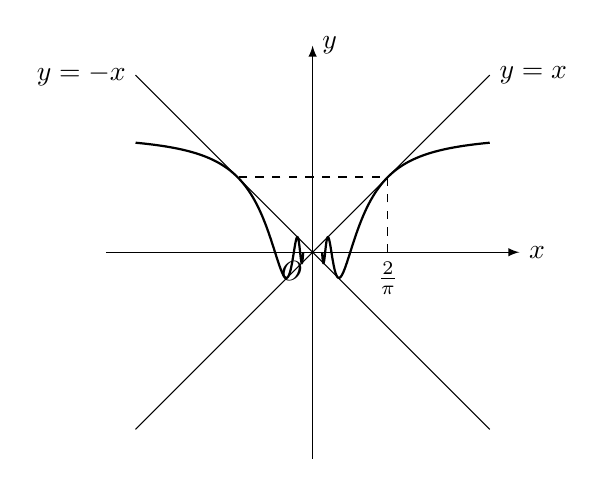
\begin{tikzpicture}[>=latex, scale=1.5]
\draw[->](-1.75,0)--(1.75,0)node[right]{$x$};
\draw[->](0,-1.75)--(0,1.75)node[right]{$y$};
\draw(-1.5,-1.5)--(1.5,1.5)node[right]{$y=x$};
\draw(-1.5,1.5)node[left]{$y=-x$}--(1.5,-1.5);
\draw[domain=0.08:1.5, samples=1000, thick]plot(\x, {\x*sin(1/\x r)});
\draw[domain=0.08:1.5, samples=1000, thick]plot(-\x, {\x*sin(1/\x r)});
\node at (0,0)[below left]{$O$};
\draw[dashed](2/pi,0)node[below]{$\frac{2}{\pi}$}--(2/pi,2/pi)--(-2/pi,2/pi);
\end{tikzpicture}
    \caption{}
\end{figure}


如果把上面的函数$f$加以扩充,即我们定义一个新函数$g$:
\[g(x)=\begin{cases}
    x\sin\frac{1}{x},& x\ne 0\\
    0,& x=0
\end{cases}\]
那么我们便得到一个在$x=0$处的连续函数.
\end{solution}

\begin{blk}
    {定义3} $\Lim_{x\to a}f(x)$存在,但不等于$f(a)$, 或者$f(a)$没有定义,则称$f$在$a$处有\textbf{可去间断点}.
\end{blk}

例1.16中的$x=0$就是$f$的可去间断点.

由函数在某一点连续的概念可以直接导出连续函数的一个重要性质如下:

\begin{blk}
{定理} 若函数$f(x)$在$x=a$连续,且$f(a)>0$, 则存在一个$a$的$\delta$邻域$(a-\delta,a+\delta)$, 使得对于每一个$x\in (a-\delta,a+\delta)$, $f(x)$都是正的.    
\end{blk}

\begin{proof}
    因为$\Lim_{x\to a} f(x)=f(a)>0$, 所以对于
$\varepsilon=\frac{1}{2}f(a)$, 必定存在一个$\delta$使得$|x-a|<\delta$时,有
\[f (x) > f (a) -\frac{1}{2}f (a) =\frac{1}{2}f (a) > 0\]
\end{proof}

\subsection{连续函数的运算}
连续函数的概念是函数概念和极限概念一个自然结合,由本章函数极限算法定理直接得出下面定理.

\begin{blk}
 {定理1} 设$f$和$g$在$a$处连续,则
 \begin{enumerate}
     \item $f\pm g$在$a$处连续;
     \item $f\cdot g$在$a$处连续;
     \item $\frac{1}{g}$在$a$处连续(若$g(a)\ne 0$);
     \item $\sqrt[n]{f}$在$a$处连续(若$f(a)>0$).
 \end{enumerate}
\end{blk}

\begin{proof}
\begin{enumerate}
    \item 因为$f$和$g$在$a$处连续,所以
    \[\Lim_{x\to a} f (x) =f (a) ,\qquad  \lim_{x\to a} g (x) =g (a)\]
    根据函数极限算法定理,得
   \[\begin{split}
    \Lim_{x\to a} (f\pm g)(x)=\Lim_{x\to a}[f(x)\pm g(x)]&=\Lim_{x\to a} f(x)\pm \Lim_{x\to a}g(x)\\
    &=f(a)\pm g(a)=(f\pm g)(a)
   \end{split} \]
    这正好就是断言$f+g$在$a$处连续.
    \item \[\begin{split}
        \Lim_{x\to a} (f\cdot g) (x)=\Lim_{x\to a}f(x)\cdot g(x)&=\Lim_{x\to a} f(x)\cdot\Lim_{x\to a}g (x)\\
        &=f (a) \cdot g (a) =(f\cdot g) (a) 
    \end{split}\]
    即$f\cdot g$在$a$处连续.
    \item 由于$g(a)\ne 0$, 又$g$在$a$处连续,根据定理,知道存在点$a$的$\delta$邻域,使得对于每一个$x\in (a-\delta,a+\delta)$,有$g(x)\cdot g(a)>0$,因此
\[\Lim_{x\to a} \frac{1}{g}(x)=\frac{1}{\Lim_{x\to a} g(x)}=\frac{1}{g(a)}=\frac{1}{g}(a)\]

\item 证明留给读者.
\end{enumerate} 
\end{proof}

在第四册下,我们根据定理证明了一些基本初等函数在其定义域上到处连续的命题,现在总结如下:

\begin{blk}
   {命题1} 任何多项式函数到处连续. 
\end{blk}

\begin{blk}{命题2}
    若$f$和$g$是两个多项式,$g\ne 0$, 那么有理函数$r=f/g$, 除去$g$的零点集合,函数$r$是有定义的,而且在其定义域上到处连续.
\end{blk}

\begin{blk}
   {命题3} $n$次算术方根函数$\sqrt[n]{x}$在$[0,+\infty)$上到处连续.
\end{blk}

因为每一个无理数可以用两串有理数数列从左、右两方面去逼近它,同样无理指数幂也可以用相应的有理指数幂去逼近它,我们用逼近法定义了无理指数幂,从而把有理指数函数开拓为在实数域上到处连续的实指数函数,于是得到下面的命题. 

\begin{blk}
    {命题4} 指数函数$a^x\; (a>0,\; a\ne 1)$到处连续.
\end{blk}

由反函数连续定理,直接得到

\begin{blk}
    {命题5} 对数函数$\log_a x$在$(0,+\infty)$上到处连续.
\end{blk}

现在将继续证明另外一些基本初等函数连续性的命题.

\begin{blk}
    {命题6} 三角函数$\sin x$和$\cos x$到处连续.
\end{blk}

\begin{proof}
设$x_0$是任意给定的实数,由三角函数的和差化积公式,得到
\[|\sin x-\sin x_0|=2\left|\sin\frac{x-x_0}{2}\right| \cdot \left|\cos \frac{x+x_0}{2}\right|\]
因为$\left|\cos\frac{x+x_0}{2}\right|\le 1$, 并根据引理得到
\[|\sin x-\sin x_0|\le 2\left|\frac{x-x_0}{2}\right|\]
即
\[|\sin x-\sin x_0|\le \left|x-x_0\right|\]
当$x\to x_0$时,$|x-x_0|\to 0$, 从而$|\sin x-\sin x_0|\to 0$, 即
\[\lim_{x\to x_0} \sin x=\sin x_0\]
因为$x_0$是任意一点,所以$\sin x$到处连续.

同样证明,得到:当$x\to x_0$时,
\[|\cos x-\cos x_0|\le |x-x_0|\to 0\]
即
\[\lim_{x\to x_0} \cos x=\cos x_0\]
因此,$\cos x$到处连续.
\end{proof}
 
由反函数连续性定理直接得出下面命题.

\begin{blk}
    {命题7} 反三角函数$y=\arcsin x\; \left(-\frac{\pi}{2}\le x\le \frac{\pi}{2}\right)$,\quad $y=\arccos x\; \left(0\le x\le \pi\right)$,\quad $y=\arctan x\; \left(-\frac{\pi}{2}< x< \frac{\pi}{2}\right)$,\quad $y=\arccot x\; \left(0<x<\pi\right)$在它们各自的定义域上到处连续.
\end{blk}

\begin{blk}{命题8}
幂函数$x^{\alpha}$($\alpha$是任何一个实数)在开区间$(0,+\infty)$上到处连续.
\end{blk}

\begin{proof}
为确定起见,假设$\alpha>0$, $n$是任何一个大于$\alpha$的整数
\[(x+h)^{\alpha} -x^{\alpha}=x^{\alpha} \left[ \left(1+\frac{h}{x}\right)^{\alpha} -1\right] \]

若$h>0$, 则$\left(1+\frac{h}{x}\right)^{\alpha} >1$,(实指数幂性质),并且
\begin{equation}
    1<\left(1+\frac{h}{x}\right)^{\alpha}<\left(1+\frac{h}{x}\right)^{n}\quad \text{(指数函数单调性)}
\end{equation}

若$h<0$, 将上面不等式方向反向,得到
\begin{equation}
    \left(1+\frac{h}{x}\right)^{n}<\left(1+\frac{h}{x}\right)^{\alpha}<1
\end{equation}
因为$\left(1+\frac{h}{x}\right)^{n}$是关于$h$的$n$次多项式,并且显然当$h\to 0$时,
\[\left(1+\frac{h}{x}\right)^{n}\to 1\]

于是,由不等式(1.10)和(1.11), 得到当$h\to 0$时,$\left(1+\frac{h}{x}\right)^{n}\to 1$. 因此
\[\lim_{h\to 0}\left[(x+h)^{\alpha}-x^{\alpha}\right]=0\]
即:
\[\lim_{h\to 0}(x+h)^{\alpha}=x^{\alpha}\]
这就是说$x^{\alpha}$在$(0,+\infty)$上处处连续.
\end{proof}

下面介绍常用的复合函数连续性定理.
\begin{blk}
{定理2} 设$X$、$Y$、$Z$是实数集,函数$g:\,X\mapsto Y$, $f:\, g(X)(\subset Y)\mapsto Z$, 又$h:\, X\mapsto Z$定义为$f$和$g$的复合函数,即$h(x)=f (g (x) )\;  (x\in X)$.

若$y=g(x)$在$x=a$处连续;$z=f(y)$在$y=g(a)=b$处连续,那么复合函数$z=h(x)=f(g(x))$在点$a$处也连续.
\end{blk}

\begin{proof}
由于
\begin{equation}
    \lim_{x\to a} g(x)=g(a)=b,\qquad x\in X
\end{equation}    
又因为:
\begin{equation}
    \lim_{y\to b} f(y)=f(b),\qquad y\in g(X)\subset Y
\end{equation}

$\therefore\quad \Lim_{x\to a}h(x)=\Lim_{x\to a}f(g(x))=\Lim_{y\to b}f(y)=f(b)=f(g(a))=h(a)$

这就说明复合函数在点$a$的连续性.
\end{proof}

把上面的等式写成
\[\lim_{x\to a}f (g (x) ) =f (g (a) ) =f \left(\lim_{x\to a} g(x) \right)\]
这个等式表示可以这样求复合函数的极限$\Lim_{x\to a}f(g(x))$, 
如果内层函数$g(x)$在点$a$的极限存在,即$\Lim_{x\to a}g(x)=b$, 
而且$f$在点$b$连续,就可以把极限符号$\Lim_{x\to a}$与函数符号$f$互换,
也就是把极限运算移到内层函数上去施行.

\begin{example}
    说明$h(x)=\sqrt[4]{\frac{1}{1+x^2}}$到处连续,并求$\Lim_{x\to a}h(x)$
\end{example}

\begin{solution}
    $h(x)=\sqrt[4]{\frac{1}{1+x^2}}$可以看作$y=g(x)=\frac{1}{1+x^2},\; x\in\mathbb{R}$
和$z=f(y)=\sqrt[4]{y},\; y\in [0,+\infty)$的复合函数.

由于$g(x)=\frac{1}{1+x^2}$在$\mathbb{R}$上到处连续并且它的值域
\[g(\mathbb{R})=(0,1]\subset [0,+\infty)=Y\]
又幂函数$f(y)=\sqrt[4]{y}$在$Y=[0,+\infty)$上到处连续,因此$f(y)=\sqrt[4]{y}$在$g(\mathbb{R})=(0,1]$上也到处连续,于是
\[\lim_{x\to a}h(x)=h\left(\lim_{x\to a}g(x)\right)=\sqrt[4]{\frac{1}{1+a^2}}\]
\end{solution}


\begin{example}
    求$\Lim_{x\to 2}\sqrt{\frac{1-\cos\pi x}{4-x^2}}$
\end{example}

\begin{solution}
设$y=g(x)=\frac{1-\cos\pi x}{4-x^2}\; (x\ne \pm 2)$,$z=f(y)=\sqrt{y}\; (y\ge 0)$,且知$f$在$[0,+\infty)$上到处连续,于是
\[f(g(x))=\sqrt{\frac{1-\cos\pi x}{4-x^2}}\]
因此:
\[\begin{split}
    \lim_{x\to 2}g(x)&=\lim_{x\to 2}\frac{1-\cos \pi x}{4-x^2}\\
    &=\lim_{x\to 2}\frac{2\sin^2\frac{\pi}{2}x}{4-x^2}=\lim_{x\to 2}\frac{\pi\sin^2\frac{\pi}{2}(2-x)}{\frac{\pi}{2}(2-x)(2+x)}\\
    &=\lim_{x\to 2}\left[\frac{\sin\frac{\pi}{2}(2-x)}{\frac{\pi}{2}(2-x)}\cdot \frac{1}{2+x}\cdot \sin\frac{\pi}{2}(2-x)  \right]\\
    &=1\cdot \frac{1}{4}\cdot 0=0\in [0,+\infty)
\end{split}\]

$\therefore\quad \Lim_{x\to 2}\sqrt{\frac{1-\cos\pi x}{4-x^2}}=\sqrt{\Lim_{x\to 2}\left(\frac{1-\cos\pi x}{4-x^2}\right)}=\sqrt{0}=0$
\end{solution}

\begin{example}
    求$\Lim_{x\to 0}\frac{\arcsin x}{x}$
\end{example}

\begin{solution}
设$\alpha=\arcsin x$,这里$-1\le x\le 1$,$-\frac{\pi}{2}\le\alpha\le \frac{\pi}{2}$,
于是,$\sin\alpha=x$.

根据反正弦函数的连续性,有
\[\lim_{x\to 0} \alpha=\lim_{x\to 0}\arcsin x=\arcsin 0=0\]
进行变量替换,得到
\[\lim_{x\to 0} \frac{\arcsin x}{x}=\lim_{x\to 0}\frac{\alpha}{\sin\alpha}=1\]
\end{solution}

下面根据指数函数与对数函数的连续性,我们要建立几个重要的极限:
\begin{enumerate}
    \item $\Lim_{x\to 0} \frac{\ln(1+x)}{x}=1$,\quad 这里$\ln$表示$\log_e$
    \item $\Lim_{x\to 0}\frac{e^x-1}{x}=1$
    \item $\Lim_{x\to 0}\frac{(1+x)^\alpha -1}{x}=\alpha$
\end{enumerate}

\begin{proof}
\begin{enumerate}
    \item $\Lim_{x\to 0} \frac{\ln(1+x)}{x}=\Lim_{x\to 0} \ln(1+x)^{1/x}$
    因为右端在对数号下的式子当$x\to 0$趋向于$e$, 所以根据对数函数的连续性,得到
\[\Lim_{x\to 0} \frac{\ln(1+x)}{x}=\Lim_{x\to 0} \ln(1+x)^{1/x}=\ln e=1\]
\item 令$e^x-1=y$, 于是当$x\to 0$时,由指数函数连续性有$y\to 0$, 其次,我们有$x=\ln(1+y)$, 因此,有
\[\Lim_{x\to 0}\frac{e^x-1}{x}=\Lim_{y\to 0}\frac{y}{\ln(1+y)}=\Lim_{y\to 0}\frac{1}{\ln(1+y)^{1/y}}=1\]
\item 我们令$(1+x)^{\alpha}-1=y$, 当$x\to 0$时,由幂函数的连续性,也有$y\to 0$, 在等式$(1+x)^{\alpha}=1+y$的两边取对数得到
\[\alpha\ln (1+x) =\ln (1+y) \]
利用这一关系式,我们把所给的表达式变形为
\[\frac{(1+x)^\alpha-1}{x}=\frac{y}{x}=\frac{y}{\ln(1+y)}\cdot \alpha\cdot\frac{\ln(1+x)}{x}\]
因此:
\[\Lim_{x\to 0} \frac{(1+x)^\alpha-1}{x}=   \Lim_{x\to 0} \frac{y}{\ln(1+y)}\cdot \alpha\cdot   \Lim_{x\to 0}  \frac{\ln(1+x)}{x}=\alpha\]
\end{enumerate}
\end{proof}

我们讨论了下面的函数:
\begin{enumerate}
    \item $f(x)=c$\quad ($c$为常数)
    \item $x^n$\quad($n$是整数)
    \item $\sqrt[n]{x}\quad (x\ge 0)$
    \item $a^n\quad (a>0,\; n\ne 1)$
    \item $\log_a x$
    \item $x^\alpha$\quad ($\alpha$是任意实常数)
    \item $\sin x,\; \cos x, \; \tan x,\; \cot x$
    \item $\arcsin x,\; \arccos x, \; \arctan x,\; \arccot x$
\end{enumerate}
上面这些函数统称为\textbf{基本初等函数}.

凡是由基本初等函数及常数,经过有限次四则运算(加、减、乘、除)及有限次函数复合的步骤而得到的且由一个式子表示的函数,及可以化为这种形式的函数,统称为\textbf{初等函数}.

例如,下列函数都是初等函数:
\begin{enumerate}
    \item $f(x)=x\sin\frac{1}{x}+2^x\log_2 x$
    \item $\varphi(x)=\arctan\frac{1}{x}+\sin(x^2+1)$
\end{enumerate}

连续函数的四则运算定理,复合函数连续性定理及反函数连续性定理,在研究初等函数的连续性时具有重要作用.现在根据这些定理,立即得到一个重要结论:

\begin{blk}
 {定理} 一切初等函数在它有定义的任何区间内到处连续.
\end{blk}

\begin{ex}
\begin{enumerate}
    \item 试证 $y=|x|$是一个到处连续的函数.
    \item 说明下列函数到处连续:
\begin{multicols}{2}
\begin{enumerate}
    \item $f(x)=\frac{x^2}{1+x^2}$
    \item $f(x)=\sin|x|$
    \item $\varphi(x)=|\sin x|$
    \item $k(x)=\left\{\cos x-\sin|x|\right\}^3$
\end{enumerate}
\end{multicols}

\item 求出下列函数的间断点,并指出其类型.
\begin{multicols}{2}
\begin{enumerate}
    \item $f(x)=\frac{1}{x-2}$
    \item $f(x)=\frac{x-1}{x^2-1}$
    \item $h(x)=x\cos^2 \frac{1}{x}$
    \item $y=\frac{1}{\sin\pi x}$
    \item $y=\tan(x-1)$
    \item $y=\frac{\sin x}{|x|}$
    \item $f(x)=\begin{cases}
        \frac{\sin x}{|x|},&x\ne 0\\
        1,& x=0
    \end{cases}$
    \item $f(x)=\cot\frac{1}{x}$
    \item $f(y)=\begin{cases}
        \cos\frac{\pi x}{2},& |x|\le 1\\
        |x-1|,& |x|>1
    \end{cases}$
\end{enumerate}
\end{multicols}
\item 试证明下列函数在其定义域内是连续的:
\begin{enumerate}
    \item $f(x)=\begin{cases}
        x^2\sin\frac{1}{x},&x\ne 0\\
        0,&x=0
    \end{cases}$
    \item $\varphi(x)=\begin{cases}
        1-x,& x<0\\
        2x^2+1,& x=0\\
        2+(x-1)^3,& x>0
    \end{cases}$
\end{enumerate}
\item 求下列变量的极限:
\begin{multicols}{2}
    \begin{enumerate}
\item $\Lim_{x\to+\infty}\left(\sin\sqrt{x+1}-\sin\sqrt{x}\right)$
\item $\Lim_{x\to 1}\frac{1+\cos\pi x}{\tan^2 \pi x}$
\item $\Lim_{x\to 0}\frac{x\sin x}{1-\cos x}$
\item $\Lim_{x\to 0}\frac{x}{\sqrt{1-\cos x}}$
\item $\Lim_{x\to 0}\frac{\cos x-\cos 3x}{x^2}$
\item $\Lim_{x\to \tfrac{\pi}{4}}\tan 2x\tan\left(\frac{\pi}{4}-x\right)$
\item $\Lim_{h\to 0}\frac{\arctan (x+h)-\arctan x}{h}$
\item $\Lim_{x\to \infty}\arcsin \frac{1-x}{1+x}$
\item $\Lim_{x\to 0}\frac{1+\sin x-\cos x}{1+\sin px-\cos px}$
\item $\Lim_{x\to 0}\frac{\log_p(1+x)}{x}$
\item $\Lim_{x\to 0}\frac{a^x-1}{x}$
\item $\Lim_{n\to \infty}n\left(\sqrt[n]{x}-1\right)$
    \end{enumerate}
\end{multicols}
\end{enumerate}
\end{ex}

\subsection{闭区间上的连续函数的性质}

我们在一中已经定义了闭区间上连续函数的意义.对于这类函数,我们要介绍它的几个重要性质.

\begin{blk}
    {中间值定理} 设$y=f(x)$是一个在闭区间$[a,b]$上到处连续的函数,设$c$是一个介于$f(a)$和$f(b)$之间的常数,则必须存在一个介于$a$、$b$之间的实数$x_0$, 使得$f(x_0)=c$.
\end{blk}

用几何术语来说,$y=f(x),\; a\le x\le b$的图象是一条连结$P(a,f(a))$点和$Q(b,f(b))$点的连续曲线,而$P$、$Q$分居于直线$y=c$的两侧,则曲线$y=f(x),\; a\le x\le b$至少和直线$y=c$有一个交点($x_0,\; f(x_0)=c$).(图1.14).
\begin{figure}[htp]
    \centering
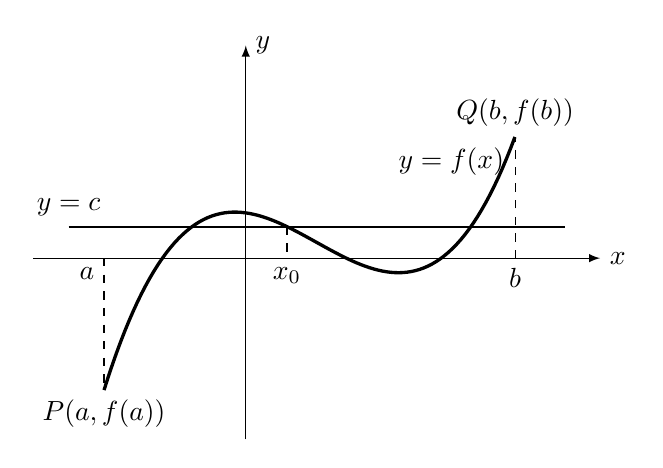
\begin{tikzpicture}[>=latex, xscale=1.8]
\draw[->](-1,-.2)--(3,-.2)node[right]{$x$};
\draw[->](.5,-2.5)--(.5,2.5)node[right]{$y$};
\draw[very thick, domain=-.5:2.4, samples=100]plot(\x, {\x*(\x-1)*(\x-2)})node[below left]{$y=f(x)$};
\draw[dashed](-.5,-.2)node[below left]{$a$}--(-.5,-1.875)node[below]{$P(a,f(a))$};
\draw[dashed](2.4,-.2)node[below]{$b$}--(2.4,1.344)node[above]{$Q(b,f(b))$};
\draw[thick](-.75,.2)node[above]{$y=c$}--(2.75,.2);
\draw[dashed](0.7909,.2)--(0.7909,-.2)node[below]{$x_0$};

\end{tikzpicture}
    \caption{}
\end{figure}


对这个定理,我们在第四册中利用二分逼近法及连续函数的性质给出了它的证明,这里不再重述.

\begin{blk}
 {最大值、最小值} 在闭区间$[a,b]$上连续的函数$f$一定在该区间上取到一个最大值和最小值.  
\end{blk}

我们先利用连续函数的图象来直观地说明这个性质,然
后用证明中间值定理的同样方法来证明这个定理.初学者可略过定理的证明,这不影响对本书后面内容的学习.

从图1.15可以看出,在$[a,b]$中,能够找到两点$x_1,x_2$使$f(x_1)=M$, $f(x_2)=m$, 而对于$[a,b]$中所有的$x$, 都有
\[m=f(x_2)\le f(x)\le f(x_1)=M\]


\begin{figure}[htp]
    \centering
    \begin{minipage}[t]{0.48\textwidth}
    \centering
    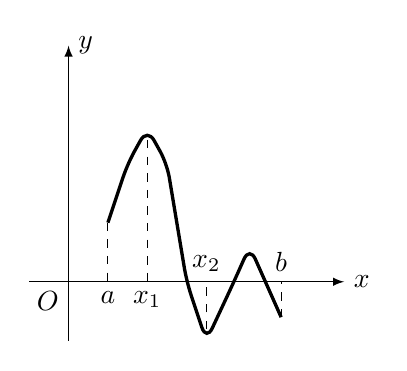
\begin{tikzpicture}[>=latex, yscale=1.5]
\draw[->](0,0)--(4,0)node[right]{$x$};
\draw[->](.5,-.5)--(.5,2)node[right]{$y$};
\draw[rounded corners=5pt, very thick](1,.5)--(1.25,1)--(1.5,1.3)--(1.75,1)--(2,0)--(2.25,-.5)--(2.6,0)--(2.8,.3)--(3,0)--(3.2,-.3);
\draw[dashed](1,.5)--(1,0)node[below]{$a$};
\draw[dashed](3.2,-.3)--(3.2,0)node[above]{$b$};
\draw[dashed](1.5,1.2)--(1.5,0)node[below]{$x_1$};
\draw[dashed](2.25,-.4)--(2.25,0)node[above]{$x_2$};
\node at (.5,0)[below left]{$O$};

    \end{tikzpicture}
    \caption{}
    \end{minipage}
    \begin{minipage}[t]{0.48\textwidth}
    \centering
    \begin{tikzpicture}[>=latex, scale=1.5]
\draw[->](-.5,0)--(2,0)node[right]{$x$};
\draw[->](0,-.5)--(0,2)node[right]{$y$};
\draw(1,0)node[below]{1}--(1,.1);
\draw(0,1)node[left]{1}--(.1,1);
\node at (0,0)[below right]{$O$};
\draw[very thick](0,0)--(1,1);
\tkzDefPoints{0/0/O, 1/1/A}
\tkzDrawPoints(O,A)
    \end{tikzpicture}
    \caption{}
    \end{minipage}
  \end{figure}


\begin{rmk}
    这个定理是假定$f$在整个闭区间上连续,如果在一点不连续,则定理的结论就可能不成立.
\end{rmk}

例如,函数$f(x)=x-[x]$, $x\in [0, 1]$在$x=1$这一点不连续,它的图象如图1.16, 我们要说明它有最小值0, 而无最大值.

事实上,$f$是分段函数:
\[f(x)=\begin{cases}
    x,& 0\le x<1\\
    0,& x=1
\end{cases}\]
$f$在$[0, 1)$上递增,故
$f(0)=f(1)=0$最小.又在$[0, 1]$上没有一点的函数值为1, 但是对于任何一个小于1的正数$k$, 恒有
\[f (k) =k- [k] =k<1\]
这就说明了$f$在$[0, 1]$上有上界1, 但始终达不到1, 现在我们进一步说明1是它的最小上界,假设定数$k'<1$是$f$在
$[0, 1]$上的上界,我们在$(k',1)$内任意取一个数$x$, 于是
\[f (x) =x- [x] =x> k'\]
这与假设$k'$是$f$在$[0, 1]$上的上界矛盾,因此1是$f$在$[0, 1]$上的最小上界,但是它不属于$f$的值域,这就说明了$f$无最大值.

从这个例中还可以看出,定理中的闭区间不能用开区间来代替.

现在给出定理的证明如下:

\begin{proof}
令$A_1=a$, $B_1=b$, $S_1=\{f(x)|x\in [a,b]\}$,设$K$是$S_1$的最小上界,记$K=l.u.b\{S_1\}$. 再令
\[S_1'=\left\{f (x) ; \; x\in \left[a,\frac{a+b}{2}\right]\right\},\quad S_1''=\left\{f(x);\; x\in\left[\frac{a+b}{2},b\right]\right\}\]
显然有:
\[S_1=S_1'\cup S_1''\]
由此不难看到:
\[K=l.u.b \{S_1\} =\max \left(l.u,b \{S'_1\} ,l.u.b\{S_1''\}\right)\]
所以$l.u.b\{S_1'\}$和$l.u.b\{S_1''\}$两者之中,至少有一个等于$K$, 换句话说,我们总可以在$[A_1,B_1]$的两个半段之中,选取其一为$[A_2,B_2]$, 使得
\[l.u.b \{S_2\} =K,\qquad  S_2= \{f (x) ,\; x\in [A_2, B_2] \}\] 
如此逐步二分,每次由$[A_{n} ,B_{n}]$归纳地选取其半段作为$[A_{n+1} ,B_{n+1}]$,使得
\[\begin{split}
    l.u.b \{f (x) ;\; x\in  [A_{n+1}, B_{n+1}] \}&=l.u.b \{f (x) ;\; x\in [A_n, B_n] \}\\
&=\cdots\\
&=l.u.b \{f (x) ;\; x\in  [a,b] \}=K.
\end{split}\]
对$\{A_n\},\{B_n \}$, 根据实数的连续性,知存在$c$使得$c\in [A_n,B_n]$, $n=1, 2, 3,\ldots$, 且$B_n-A_n\to 0$.

现在我们要再利用$f(x)$到处连续这一性质,说明$f(c)=K$. 假若不然,即$f(c)<K$,则可以取$\varepsilon=\frac{1}{2}(K-f(c))>0$,然后利用$f(x)$在$c$点的连续性,知存在点$c$的$\delta$邻域,使得当$|x-c|<\delta$时,有
\[|f(x)-f(c)|<\varepsilon\]
即:
\[\begin{split}
    f(x)<f(c)+\varepsilon&=f(c)+\frac{1}{2}K-\frac{1}{2}f(c)\\
    &=\frac{1}{2}[K+f(c)]\\
    &=\frac{1}{2}[K+K-2\varepsilon]=K-\varepsilon
\end{split}\]
所以
\[l.u.b \{f (x) ;\; x\in  (c-\delta,c+\delta) \} \le K-\varepsilon\]
但是,由$\Lim_{n\to\infty} A_n=\Lim_{n\to\infty}B_n=c$, 知当$n$足够大时,有
\[[A_n,B_n]\subset (c-\delta,c+\delta)\]
这显然和$[A_n,B_n]$的选取法,亦即保持
\[l.u.b \{f (x) ;\; x\in [A_n,B_n]\}=K\]
相矛盾,因此,$f(c)$必须等于$K$. 

类似地,可以证明存在使函数$f$达到它的最小值的一个点.
\end{proof}

\subsection*{习题1.2}
\begin{enumerate}
    \item 求下列函数的极限:
\begin{enumerate}\begin{multicols}{2}
    \item $\Lim_{x\to 0}(\cos x)^{\sin x}$
    \item $\Lim_{x\to 0}\frac{\frac{x^2}{e^{2x}}}{\ln\left(1+\frac{x^2}{e^{2x}}\right)}$
    \item $\Lim_{x\to 0}\frac{\frac{x^2}{e^{2x}}}{\sin^2 \frac{x}{e^{x}}}$
    \item $\Lim_{x\to \infty}n^2\left(-x^{\tfrac{1}{n}}-x^{\tfrac{1}{n+1}}\right)$
    \item $\Lim_{x\to 0}\frac{\left(e^x+e^{-x}\right)\left(e^x-e^{-x}\right)}{2x}$
    \item $\Lim_{x\to 0}(1-2x)^{\tfrac{1}{x}}$
    \item $\Lim_{x\to \infty}10\left(1+\frac{0.03}{n}\right)^n$
    \item $\Lim_{x\to +\infty}\arccos\left(\sqrt{x^2+x}-x\right)$
    \item $\Lim_{x\to -\infty}\arctan\frac{x-4}{(x-2)^2}$
    \item $\Lim_{x\to -\infty}\arctan\frac{x}{\sqrt{1+x^2}}$
    \item $\Lim_{x\to -\infty}\frac{x}{\sqrt{1+x^2}}$
\end{multicols}   
    \item $\Lim_{x\to 0}\frac{\ln\frac{1+x}{1-x}}{\arctan(1+x)-\arctan(1-x)}$
\end{enumerate} 

\item 在一个以弦$AB$为界的弓形中,把点$A$与$B$与弧$\wideparen{AB}$的中点$C$用直线连结起来,于是得到一个等腰三角形$\triangle  ABC$, 再在$A$与$B$作切线,它们交于$D$, 试计算$\Lim_{x\to 0}\frac{\triangle ABC}{\triangle ABD}$,其中$x$是
弦$AB$所对应的中心角.

\item $f(x)=\frac{ax^3+bx^2+cx+d}{x^2-x-2}$满足条件
\[\lim_{x\to \infty} f(x)=2,\qquad \lim_{x\to 2} f(x)=3\]
求$f(x)$.
\end{enumerate}

